\documentclass{article}
\usepackage{iclr2026_conference,times}
% \iclrfinalcopy omitted for double-blind review.

\input{math_commands.tex}

\usepackage{hyperref}
\usepackage{url}
\usepackage{microtype}
\usepackage{graphicx}
\usepackage{booktabs}
\usepackage{amsmath}
\usepackage{amssymb}
\usepackage{amsthm}
\usepackage{enumitem}
\usepackage{xcolor}
\usepackage{longtable}
\setlist{nosep, topsep=3pt, partopsep=0pt}
\hypersetup{pdfauthor={},pdftitle={},colorlinks=true,linkcolor=blue,citecolor=blue,urlcolor=blue}

\newtheorem{theorem}{Theorem}
\newtheorem{proposition}{Proposition}
\newtheorem{corollary}{Corollary}
\newtheorem{lemma}{Lemma}
\newtheorem{fact}{Fact}
\theoremstyle{definition}
\newtheorem{definition}{Definition}
\newtheorem{remark}{Remark}

\renewcommand{\topfraction}{0.92}
\renewcommand{\bottomfraction}{0.92}
\renewcommand{\textfraction}{0.05}
\renewcommand{\floatpagefraction}{0.80}
\setlength{\textfloatsep}{8pt plus 2pt minus 2pt}
\setlength{\abovecaptionskip}{4pt}
\setlength{\belowcaptionskip}{2pt}

\newcommand{\dgm}{\mathrm{dgm}}
\newcommand{\VR}{\mathrm{VR}}
\newcommand{\defect}{\delta}
\newcommand{\stw}{S}

\newcommand{\NSettings}{11}
\newcommand{\NModels}{5}
\newcommand{\NCellsTotal}{568,028}
\newcommand{\NSinkSettings}{10}
\newcommand{\PctConedRange}{36--88\%}
\newcommand{\SinkMassRange}{0.42 to 0.69}
\newcommand{\NoSinkMass}{0.02}
\newcommand{\RhoMin}{0.999}
\newcommand{\RhoNoSink}{0.967}
\newcommand{\RhoDeltaHone}{0.33 to 0.89}
\newcommand{\NViolations}{0}
\newcommand{\MaxSeedSD}{0.008}
\newcommand{\NComp}{10}
\newcommand{\NTOneEquiv}{4}
\newcommand{\TOneRange}{-0.015 to +0.031}
\newcommand{\TTwoRange}{+0.004 to +0.030}
\newcommand{\NTTwoEquiv}{3}
\newcommand{\TThreeTQA}{+0.032 to +0.045}
\newcommand{\TThreeOnp}{+0.002 to +0.029}
\newcommand{\TThreeHE}{+0.052 to +0.055}
\newcommand{\NTFourEquiv}{8}
\newcommand{\TFourRange}{-0.008 to +0.026}
\newcommand{\PHTopoRange}{-0.001 to +0.011}
\newcommand{\NPHTopoEquiv}{9}
\newcommand{\NPHTopoTotal}{9}
\newcommand{\PHEntRange}{-0.016 to +0.036}
\newcommand{\NIZeroEquiv}{10}
\newcommand{\NIZeroTotal}{10}
\newcommand{\IZeroRange}{0.000 to +0.001}
\newcommand{\NIDeflEquiv}{10}
\newcommand{\IDeflRange}{-0.001 to +0.002}
\newcommand{\LexTQA}{0.82}
\newcommand{\LexOnp}{0.60 to 0.74}
\newcommand{\LexHE}{0.98}
\newcommand{\LogpTQA}{0.58 to 0.64}
\newcommand{\LogpOnp}{0.72 to 0.88}
\newcommand{\ZeroDTQA}{0.58 to 0.75}
\newcommand{\ZeroDOnp}{0.71 to 0.73}
\newcommand{\ZeroDHE}{0.79 to 0.82}
\newcommand{\NonTopoAll}{0.84 to 0.94}
\newcommand{\HiddenAll}{0.83 to 0.93}
\newcommand{\LookbackAll}{0.82 to 0.90}
\newcommand{\HiddenHE}{1.00}
\newcommand{\SplitConed}{-0.001 to +0.004}
\newcommand{\SplitOpen}{+0.003 to +0.029}
\newcommand{\OnpAccRange}{26\% to 56\%}

\newcommand{\SinkTableTheory}{%
\begin{tabular}{llrrrrrrrr}
\toprule
Benchmark & Model & $\bar N$ & graphs & viol. & sink attn. & coned & $H_1{=}\emptyset\,|\,$coned & $\rho_{\text{raw}}$ & $\rho_{/N}$ \\
\midrule
TruthfulQA & Qwen2.5-3B & 44.2 & 58,824 & 0 & 0.50 & 62.2\% & 100.0\% & 1.000 & 1.000 \\
TruthfulQA & Qwen2.5-1.5B & 44.2 & 45,752 & 0 & 0.53 & 64.5\% & 100.0\% & 1.000 & 1.000 \\
TruthfulQA & Phi-3-mini & 29.0 & 52,288 & 0 & 0.69 & 88.4\% & 100.0\% & 1.000 & 1.000 \\
TruthfulQA & TinyLlama-1.1B & 42.3 & 35,948 & 0 & 0.53 & 36.2\% & 100.0\% & 1.000 & 0.982 \\
TruthfulQA & SmolLM-1.7B & 32.4 & 39,216 & 0 & 0.02 & 0.0\% & -- & 0.967 & 0.412 \\
HaluEval & Qwen2.5-3B & 126.9 & 72,000 & 0 & 0.42 & 52.7\% & 100.0\% & 1.000 & 1.000 \\
HaluEval & Qwen2.5-1.5B & 128.1 & 28,000 & 0 & 0.45 & 62.5\% & 100.0\% & 1.000 & 1.000 \\
TriviaQA (on-policy) & Qwen2.5-3B & 68.6 & 72,000 & 0 & 0.48 & 63.0\% & 100.0\% & 1.000 & 1.000 \\
TriviaQA (on-policy) & Qwen2.5-1.5B & 68.8 & 56,000 & 0 & 0.52 & 50.6\% & 100.0\% & 1.000 & 1.000 \\
TriviaQA (on-policy) & Phi-3-mini & 46.1 & 64,000 & 0 & 0.69 & 87.1\% & 100.0\% & 1.000 & 1.000 \\
TriviaQA (on-policy) & TinyLlama-1.1B & 72.0 & 44,000 & 0 & 0.50 & 36.4\% & 100.0\% & 1.000 & 0.991 \\
\bottomrule
\end{tabular}
}
\newcommand{\SinkTableAuc}{%
\begin{tabular}{lccccccccccc}
\toprule
Setting & Lex. & LogP & LLM-C. & Sink & 0D & 1D & Sink$_h$ & 0D$_h$ & Lookb. & Hidden & Non-topo. \\
\midrule
TQA Qw3B & .820 & .630 & .693 & .737 & .736 & .660 & .851 & .853 & .897 & .913 & \textbf{.926} \\
TQA Qw1.5B & .820 & .638 & .666 & .723 & .726 & .586 & .830 & .838 & .851 & .916 & \textbf{.917} \\
TQA Phi-3 & .820 & .578 & .653 & .651 & .646 & .526 & .871 & .868 & .892 & .933 & \textbf{.936} \\
TQA TinyLl. & .820 & .637 & .614 & .643 & .654 & .592 & .808 & .806 & .850 & .883 & \textbf{.885} \\
TQA SmolLM & .820 & .588 & .604 & .611 & .583 & .543 & .720 & .800 & .863 & .894 & \textbf{.899} \\
\midrule
HE Qw3B & .981 & .993 & .745 & .829 & .811 & .710 & .958 & .971 & .998 & 1.00 & \textbf{1.00} \\
HE Qw1.5B & .979 & .995 & .791 & .820 & .789 & .747 & .922 & .949 & .999 & 1.00 & \textbf{1.00} \\
\midrule
TrQA Qw3B & .596 & .839 & .688 & .717 & .732 & .601 & .820 & .807 & .861 & .841 & \textbf{.870} \\
TrQA Qw1.5B & .609 & .823 & .676 & .707 & .716 & .574 & .767 & .768 & .824 & .855 & \textbf{.873} \\
TrQA Phi-3 & .635 & .877 & .676 & .707 & .710 & .546 & .826 & .807 & .840 & .867 & \textbf{.883} \\
TrQA TinyLl. & .740 & .724 & .688 & .720 & .720 & .659 & .814 & .775 & .823 & .827 & \textbf{.842} \\
\bottomrule
\end{tabular}
}
\newcommand{\SinkTableTests}{%
\begin{tabular}{lcccccccc}
\toprule
Setting & Sink$-$0D & 0D$\mid$Sink & $P_{0,h}\mid$Sink$_h$ & Defl.$\mid$Sink & 1D$\mid$0D & 0D$\mid$NT & 0D$\oplus$NT & Defl.$\mid$NT \\
\midrule
TQA Qw3B & $+0.001$$^{\equiv}$ & $+0.003$$^{\equiv}$ & $+0.009$$^{\equiv}$ & $+0.029$$^{*}$ & $+0.033$$^{*}$ & $0.000$$^{\equiv}$ & $0.000$$^{\equiv}$ & $+0.001$$^{\equiv}$ \\
TQA Qw1.5B & $-0.003$$^{\equiv}$ & $+0.012$$^{*}$ & $+0.011$$^{\equiv}$ & $+0.034$$^{*}$ & $-0.008$$^{\equiv}$ & $0.000$$^{\equiv}$ & $0.000$$^{\equiv}$ & $0.000$$^{\equiv}$ \\
TQA Phi-3 & $+0.005$$^{\equiv}$ & $+0.006$$^{\equiv}$ & $0.000$$^{\equiv}$ & $+0.033$$^{*}$ & $-0.003$$^{\equiv}$ & $0.000$$^{\equiv}$ & $0.000$$^{\equiv}$ & $+0.001$$^{\equiv}$ \\
TQA TinyLl. & $-0.010$ & $+0.020$$^{*}$ & $+0.003$$^{\equiv}$ & $+0.045$$^{*}$ & $+0.007$$^{\equiv}$ & $0.000$$^{\equiv}$ & $0.000$$^{\equiv}$ & $-0.001$$^{\equiv}$ \\
TQA SmolLM & $+0.028$$^{*}$ & $+0.030$$^{*}$ & $+0.106$$^{*}$ & $+0.041$$^{*}$ & $+0.005$$^{\equiv}$ & $0.000$$^{\equiv}$ & $0.000$$^{\equiv}$ & $-0.001$$^{\equiv}$ \\
\midrule
HE Qw3B & $+0.018$$^{*}$ & $+0.028$$^{*}$ & $+0.004$$^{\equiv}$ & $+0.058$$^{*}$ & $+0.015$$^{*}$ & $0.000$$^{\equiv}$ & $0.000$$^{\equiv}$ & $0.000$$^{\equiv}$ \\
HE Qw1.5B & $+0.031$$^{*}$ & $+0.012$$^{*}$ & $+0.008$$^{\equiv}$ & $+0.052$$^{*}$ & $+0.026$$^{*}$ & $0.000$$^{\equiv}$ & $0.000$$^{\equiv}$ & $0.000$$^{\equiv}$ \\
\midrule
TrQA Qw3B & $-0.015$$^{*}$ & $+0.021$$^{*}$ & $+0.004$$^{\equiv}$ & $+0.002$ & $-0.003$$^{\equiv}$ & $+0.001$$^{\equiv}$ & $+0.002$$^{\equiv}$ & $0.000$$^{\equiv}$ \\
TrQA Qw1.5B & $-0.009$ & $+0.010$ & $+0.004$$^{\equiv}$ & $+0.012$ & $-0.002$$^{\equiv}$ & $0.000$$^{\equiv}$ & $0.000$$^{\equiv}$ & $-0.001$$^{\equiv}$ \\
TrQA Phi-3 & $-0.004$$^{\equiv}$ & $+0.006$$^{\equiv}$ & $+0.002$$^{\equiv}$ & $+0.029$$^{*}$ & $-0.005$$^{\equiv}$ & $0.000$$^{\equiv}$ & $0.000$$^{\equiv}$ & $+0.002$$^{\equiv}$ \\
TrQA TinyLl. & $+0.001$$^{\equiv}$ & $+0.004$$^{\equiv}$ & $-0.001$$^{\equiv}$ & $+0.014$ & $-0.002$$^{\equiv}$ & $0.000$$^{\equiv}$ & $0.000$$^{\equiv}$ & $0.000$$^{\equiv}$ \\
\bottomrule
\end{tabular}
}
\newcommand{\SinkTableOnpolicy}{%
\begin{tabular}{lrrrr}
\toprule
Model & questions & accuracy & rows used & mean answer tokens \\
\midrule
Qwen2.5-3B & 2,000 & 42.4\% & 2,000 & 5.5 \\
Qwen2.5-1.5B & 2,000 & 31.4\% & 2,000 & 5.8 \\
Phi-3-mini & 2,000 & 56.2\% & 2,000 & 6.0 \\
TinyLlama-1.1B & 2,000 & 26.4\% & 2,000 & 18.9 \\
\bottomrule
\end{tabular}
}
\newcommand{\SinkTableToha}{%
\begin{tabular}{lccccccccccccc}
\toprule
Setting & $\defect_P{=}0$ & $\rho(d,\bar\pi)$ & TOHA & TOHA$[\bar\pi]$ & TOHA$[\bar a_0]$ & TOHA$_{\text{sup}}$ & $\bar\pi_{\text{sup}}$ & $\bar a_{0,\text{sup}}$ & Non-topo. & $\bar\pi-$TOHA & $\bar a_0-$TOHA & TOHA$\oplus\bar\pi$ & TOHA$\oplus$NT \\
\midrule
TQA Qw3B & 57\% & .976 & .668 & .670 & .649 & .892 & .892 & .892 & .926 & $+0.003$$^{\equiv}$ & $-0.018$$^{*}$ & $+0.003$$^{\equiv}$ & $+0.003$$^{\equiv}$ \\
TQA Qw1.5B & 58\% & .978 & .646 & .649 & .628 & .858 & .857 & .857 & .917 & $+0.003$$^{\equiv}$ & $-0.018$$^{*}$ & $+0.005$$^{\equiv}$ & $+0.002$$^{\equiv}$ \\
TQA Phi-3 & 74\% & .996 & .751 & .742 & .715 & .898 & .901 & .905 & .936 & $-0.009$$^{*}$ & $-0.036$$^{*}$ & $0.000$$^{\equiv}$ & $0.000$$^{\equiv}$ \\
TQA TinyLl. & 74\% & .995 & .666 & .655 & .618 & .845 & .843 & .848 & .885 & $-0.012$$^{*}$ & $-0.049$$^{*}$ & $+0.002$$^{\equiv}$ & $+0.001$$^{\equiv}$ \\
TQA SmolLM & 58\% & .954 & .701 & .695 & .595 & .862 & .860 & .841 & .899 & $-0.007$$^{\equiv}$ & $-0.107$$^{*}$ & $+0.005$$^{\equiv}$ & $+0.002$$^{\equiv}$ \\
\midrule
HE Qw3B & 68\% & .987 & .967 & .982 & .961 & .999 & .999 & 1.00 & 1.00 & $+0.015$$^{*}$ & $-0.007$$^{\equiv}$ & $0.000$$^{\equiv}$ & $0.000$$^{\equiv}$ \\
HE Qw1.5B & 69\% & .988 & .970 & .988 & .972 & .999 & .999 & .999 & 1.00 & $+0.018$$^{*}$ & $+0.002$$^{\equiv}$ & $0.000$$^{\equiv}$ & $0.000$$^{\equiv}$ \\
\midrule
TrQA Qw3B & 76\% & .991 & .728 & .736 & .742 & .862 & .863 & .870 & .870 & $+0.009$ & $+0.014$$^{*}$ & $+0.002$$^{\equiv}$ & $+0.012$$^{*}$ \\
TrQA Qw1.5B & 77\% & .992 & .712 & .714 & .708 & .828 & .827 & .836 & .873 & $+0.002$$^{\equiv}$ & $-0.005$ & $+0.003$$^{\equiv}$ & $+0.004$$^{\equiv}$ \\
TrQA Phi-3 & 88\% & .998 & .724 & .731 & .733 & .847 & .851 & .850 & .883 & $+0.007$$^{\equiv}$ & $+0.008$ & $0.000$$^{\equiv}$ & $+0.001$$^{\equiv}$ \\
TrQA TinyLl. & 66\% & .994 & .714 & .725 & .693 & .833 & .826 & .832 & .842 & $+0.011$$^{*}$ & $-0.021$$^{*}$ & $+0.007$$^{\equiv}$ & $+0.010$$^{*}$ \\
\bottomrule
\end{tabular}
}
\newcommand{\SinkTableTohaCausal}{%
\begin{tabular}{lrrrrrrrr}
\toprule
Model & $b$ & $\defect_P{=}0$ & sink top & $\rho(d,1-\bar a_0)$ & TOHA & TOHA$[\bar a_0]$ & TOHA$_{\text{sup}}$ & $\bar a_{0,\text{sup}}$ \\
\midrule
Qwen2.5-1.5B & $-2$ & 37\% & 21\% & 0.605 & 0.667 & 0.624 & 0.843 & 0.849 \\
Qwen2.5-1.5B & $0$ & 58\% & 45\% & 0.893 & 0.646 & 0.628 & 0.858 & 0.857 \\
Qwen2.5-1.5B & $+2$ & 72\% & 60\% & 0.970 & 0.667 & 0.637 & 0.857 & 0.857 \\
Qwen2.5-1.5B & $+4$ & 69\% & 56\% & 0.962 & 0.647 & 0.640 & 0.839 & 0.838 \\
TinyLlama-1.1B & $-2$ & 63\% & 21\% & 0.406 & 0.698 & 0.626 & 0.845 & 0.834 \\
TinyLlama-1.1B & $0$ & 74\% & 63\% & 0.967 & 0.666 & 0.618 & 0.845 & 0.848 \\
TinyLlama-1.1B & $+2$ & 81\% & 75\% & 0.992 & 0.652 & 0.610 & 0.848 & 0.848 \\
TinyLlama-1.1B & $+4$ & 86\% & 83\% & 0.996 & 0.665 & 0.616 & 0.844 & 0.842 \\
\bottomrule
\end{tabular}
}

% sink_results.tex -- results prose. All numbers come from \newcommand{\NSettings}{11}
\newcommand{\NModels}{5}
\newcommand{\NCellsTotal}{568,028}
\newcommand{\NSinkSettings}{10}
\newcommand{\PctConedRange}{36--88\%}
\newcommand{\SinkMassRange}{0.42 to 0.69}
\newcommand{\NoSinkMass}{0.02}
\newcommand{\RhoMin}{0.999}
\newcommand{\RhoNoSink}{0.967}
\newcommand{\RhoDeltaHone}{0.33 to 0.89}
\newcommand{\NViolations}{0}
\newcommand{\MaxSeedSD}{0.008}
\newcommand{\NComp}{10}
\newcommand{\NTOneEquiv}{4}
\newcommand{\TOneRange}{-0.015 to +0.031}
\newcommand{\TTwoRange}{+0.004 to +0.030}
\newcommand{\NTTwoEquiv}{3}
\newcommand{\TThreeTQA}{+0.032 to +0.045}
\newcommand{\TThreeOnp}{+0.002 to +0.029}
\newcommand{\TThreeHE}{+0.052 to +0.055}
\newcommand{\NTFourEquiv}{8}
\newcommand{\TFourRange}{-0.008 to +0.026}
\newcommand{\PHTopoRange}{-0.001 to +0.011}
\newcommand{\NPHTopoEquiv}{9}
\newcommand{\NPHTopoTotal}{9}
\newcommand{\PHEntRange}{-0.016 to +0.036}
\newcommand{\NIZeroEquiv}{10}
\newcommand{\NIZeroTotal}{10}
\newcommand{\IZeroRange}{0.000 to +0.001}
\newcommand{\NIDeflEquiv}{10}
\newcommand{\IDeflRange}{-0.001 to +0.002}
\newcommand{\LexTQA}{0.82}
\newcommand{\LexOnp}{0.60 to 0.74}
\newcommand{\LexHE}{0.98}
\newcommand{\LogpTQA}{0.58 to 0.64}
\newcommand{\LogpOnp}{0.72 to 0.88}
\newcommand{\ZeroDTQA}{0.58 to 0.75}
\newcommand{\ZeroDOnp}{0.71 to 0.73}
\newcommand{\ZeroDHE}{0.79 to 0.82}
\newcommand{\NonTopoAll}{0.84 to 0.94}
\newcommand{\HiddenAll}{0.83 to 0.93}
\newcommand{\LookbackAll}{0.82 to 0.90}
\newcommand{\HiddenHE}{1.00}
\newcommand{\SplitConed}{-0.001 to +0.004}
\newcommand{\SplitOpen}{+0.003 to +0.029}
\newcommand{\OnpAccRange}{26\% to 56\%}
,
% which sinktda/report.py regenerates from sinktda_results/.

\newcommand{\RESULTSREDUCTION}{%
Table~\ref{tab:theory} checks Theorem~\ref{thm:cone} on every layer-level graph of every example: \NCellsTotal{} graphs in total. There are \NViolations{} violations of any bound. In the \NSinkSettings{} settings whose models place \SinkMassRange{} of attention on token~0, \PctConedRange{} of graphs are \emph{exactly} coned ($\defect_0=0$), and on every one of them $H_1$ is empty, as prediction C2 requires. Across graphs, $\defect_0$ and $1$D total persistence have Spearman correlation \RhoDeltaHone{} (C3), the floor being the \RhoDeltaHoneNearN{} settings above \RhoDeltaHoneNearCut{} coned, where both quantities are near-constant (\RhoDeltaHoneNearHOneZero{} of graphs have no $1$D bars) and the correlation is degenerate rather than weak; elsewhere it is at least \RhoDeltaHoneRest{}. Both $P_0$ and the star weight $\stw_0=(N{-}1)(1-\bar m)$ scale with sequence length, so their raw per-layer rank correlation (median $\ge$\RhoRawMin{}) partly reflects length. After dividing both by $N{-}1$, the median per-layer rank correlation between $P_0/(N{-}1)$ and $1-\bar m$ is still at least \RhoMin{} in every sink setting (C1). In most layers, then, length-normalized $0$D total persistence is, up to rank, one minus the mean attention paid to the first token. The weakest single layer per setting reaches only \RhoLayerMinRange{}.

Figure~\ref{fig:layers} shows where coning happens: in the middle of the network, where sink attention is high. The first few layers are never sink-dominated, and in some models (TinyLlama, the Qwen models) so is a block of late layers; these layers are rarely coned. There, the length-normalized correlation can drop, as Theorem~\ref{thm:cone}(b) allows once $(N{-}1)\defect_0$ is comparable to the spread of $\stw_0$ across examples.

\paragraph{Models without a first-token sink as a contrast.} Our study includes \NNoSinkModels{} models that place almost no attention on token~0 --- \NoSinkModels{}, at \NoSinkMass{} --- and none of their graphs is coned at $s=0$, so Theorem~\ref{thm:cone} at the first token gives no useful guarantee for them. They are not alike. Allowing any apex, \NoSinkConedAnyMin{} of \NoSinkConedAnyMinModel{}'s graphs are coned --- no vertex cones any of them --- against \NoSinkConedAnyMax{} of \NoSinkConedAnyMaxModel{}'s, whose attention is strongly concentrated, just not on token~0 (\S\ref{sec:toha}): one model has no cone structure to find, the other is one where $s=0$ is the wrong apex. Their $H_1$ is non-empty on \NoSinkHOneNonempty{} of graphs, and although the raw $\rho(P_0,\stw_0)$ is \RhoNoSinkRaw{}, this is almost entirely shared length: the length-normalized correlation is \RhoNoSink{}. Both differ from the sink-dominated models in weights, data and template, so this is a contrast, not a controlled intervention; the within-model intervention is deflation (C4, below). The reduction is a property of sink-dominated attention, not of the pipeline.
}

\newcommand{\RESULTSBEYOND}{%
If $0$D persistence reduced \emph{exactly} to the star, a classifier on the two sink features would match one on the two $0$D features in every layer. Table~\ref{tab:tests} (``Sink vs.\ 0D'') shows the two banks differ by \TOneRange{} AUC across the \NComp{} sink settings evaluated, and are statistically equivalent within $\pm0.015$ in \NTOneEquiv{} of them (the TOST power of this comparison is modest, so non-equivalence is not evidence of a difference). Adding $0$D to the sink bank gains \TTwoRange{}.

\paragraph{The residual lives exactly where the theory says it can.} We split layers without using labels: \emph{coned} layers ($\ge90\%$ of graphs coned) and \emph{open} layers ($<50\%$). Adding the coned layers' $0$D features to \textsc{Sink} changes AUC by \SplitConed{}, whereas the open layers account for \SplitOpen{} (Appendix~\ref{app:tables}). Almost everything $0$D adds beyond sink attention comes from the layers where the sink does not dominate.

\paragraph{Per head, the reduction is tighter.} Per-head sink mass and per-head $0$D are far stronger than their head-averaged versions (Table~\ref{tab:auc}), but adding per-head MST total ($P_{0,h}$) to per-head sink mass changes AUC by only \PHTopoRange{}, which is equivalent within $\pm0.015$ in \NPHTopoEquiv{} of the \NPHTopoTotal{} sink settings with per-head features.

\paragraph{The coning defect is a signal, but not a new one.} Theorem~\ref{thm:cone} singles out $\defect_0$ as the only place where topology can depart from the sink, so we also test it as a detector. Head-averaged, it is weak (AUC \DefLayerAuc{}). Per head it is strong (\DefHeadAuc{}), and stacked onto per-head sink mass it adds \DefHSinkRange{} AUC (95\% interval above $0$ in \DefHSinkSig{} of \DefTotal{} settings). Stacked onto the non-topological probes, however, it adds only \DefHNTRange{} (above $0$ in \DefHNTSig{}, equivalent within $\pm0.015$ in \DefHNTEquiv{} of \DefTotal{}).

\paragraph{Deleting the sink exposes some, redundant, structure.} Deflated PH (C4) adds \TThreeTQA{} over \textsc{Sink} on TruthfulQA (95\% interval excludes $0$ in \NDeflTQASig{} of \NDeflTQATotal{} sink settings) but only \TThreeOnp{} on the on-policy benchmark (\NDeflOnpSig{} of \NDeflOnpTotal{}). Answer-only PH behaves similarly (Appendix~\ref{app:tables}). So attention graphs carry some non-sink geometry, most clearly on teacher-forced text. As \S\ref{sec:detection} shows, this geometry is already available to non-topological probes.
}

\newcommand{\RESULTSONEDIM}{%
Under i.i.d.\ weights, $1$D persistence grows faster than linearly over the lengths that matter here and linearly asymptotically (Proposition~\ref{prop:morse}; Figure~\ref{fig:synthetic}, left). Real attention behaves very differently: most graphs have \emph{no} $1$D bars at all (Table~\ref{tab:theory}), and the bars that exist are confined to graphs with a non-zero coning defect. Figure~\ref{fig:synthetic} (middle) reproduces this transition in a controlled setting: raising the sink's logit bias moves random causal attention from the i.i.d.-like regime to exact coning, with $H_1$ emptying in lockstep.

This explains a recurring empirical observation, that $1$D features add little to $0$D. At full sample size, adding length-normalized $1$D to $0$D changes AUC by \TFourRange{} and is equivalent within $\pm0.015$ in \NTFourEquiv{} of \NComp{} sink settings; the exceptions are \TFourExceptions{}; of these, adding $1$D significantly improves AUC in \TFourHelps{}, while the remaining one has a negative point estimate whose interval is too wide to certify equivalence. The TruthfulQA Qwen2.5-3B gain is also the result that is most sensitive to inference precision (Appendix~\ref{app:impl}). The mechanism is not that loops are uninformative in principle. In a strongly sinked model, a loop can only exist where some token pays another token more attention than one of the two pays to the sink, and its lifetime is bounded by that excess. Figure~\ref{fig:synthetic} (right) makes this concrete. A planted $6$-cycle that $H_1$ detects easily under a moderate sink ($b{=}6$, $\gamma{=}8$: AUC \PlantModerate{}) is invisible under a strong one ($b{=}8$, $\gamma\le4$: AUC $\le$\PlantStrong{}) until it is strong enough to break the cone. Without any sink ($b{=}0$) $H_1$ also misses it (AUC $\le$\PlantNone{}), because random attention already has many background cycles; $1$D persistence is informative only in between.
}

\newcommand{\RESULTSDETECTION}{%
Table~\ref{tab:auc} places attention-graph topology among standard detectors. Three patterns hold across benchmarks.

\emph{Topology is dominated by cheap non-topological probes.} On TruthfulQA and the on-policy benchmark, a mean-pooled hidden-state probe (\HiddenAll{}) and per-head Lookback ratios (\LookbackAll{}) outperform every topological bank, and their combination with log-probability, LLM-Check, and row statistics reaches \NonTopoAll{}. Adding $0$D PH to that combination changes AUC by \IZeroRange{} (equivalent within $\pm0.015$ in \NIZeroEquiv{} of the \NIZeroTotal{} settings with per-head features), and adding sink-deflated PH changes it by \IDeflRange{} (equivalent in \NIDeflEquiv{} of \NIZeroTotal{}). Early fusion could hide a small bank inside a ${\sim}2{,}000$-dimensional one, so we repeat the test with late fusion. Stacking the $0$D score onto the non-topological score changes AUC by \LFZeroNTRange{} (equivalent in \LFZeroNTEquiv{} of \LFZeroNTTotal{} settings; the 95\% interval lies above $0$ in \LFZeroNTSig{} of them), and stacking the deflated-PH score changes it by \LFDeflNTRange{} (equivalent in \LFDeflNTEquiv{} of \LFDeflNTTotal{}).

\emph{Which cheap probe wins depends on whether text is teacher-forced.} On TruthfulQA, token log-probability is weak (\LogpTQA{}), consistent with the benchmark's design around imitative falsehoods, and $0$D PH (\ZeroDTQA{}) scores higher for \NLogpBeatsZeroDTQA{} of \NLogpZeroDTQATotal{} models, significantly so for \NLogpZeroDTQA{}. On-policy, log-probability is strong (\LogpOnp{}) and significantly beats $0$D (\ZeroDOnp{}) for \NLogpOnpSig{} of \NLogpOnpTotal{} models. Conclusions about topology versus confidence drawn from a single teacher-forced benchmark do not transfer.

\emph{Per-head resolution matters more than topology.} Per-head features of every kind are far stronger than head-averaged ones, and per-head entropy lands within \PHEntRange{} AUC of per-head $0$D (Appendix~\ref{app:tables}).
}

\newcommand{\RESULTSARTIFACTS}{%
A TF-IDF model on the answer text alone reaches \LexTQA{} AUC on TruthfulQA and \LexHE{} on HaluEval, but only \LexOnp{} on-policy: teacher-forced benchmarks reward recognizing how the dataset's answers were \emph{written} \citep{hussain2026parallax,janiak2025illusion}. We draw no conclusions from HaluEval, where lexical separability is near perfect.
}

\newcommand{\RESULTSDISCUSSION}{%
\paragraph{What attention-graph topology measures.} In decoder-only models, Vietoris--Rips persistence of an attention graph, and every stable summary of it, is controlled by one scalar per graph: the coning defect of the first token. The same is true of TOHA's prompt--response divergence, with the prompt playing the role of the apex. Where it is zero, as in most middle-layer graphs of every sink-dominated model we tested, $0$D total persistence equals $(N{-}1)(1-\bar m)$, a function of length and sink attention alone, and higher homology is empty. Where it is positive, Theorem~\ref{thm:cone} bounds how far topology can depart from the sink; in our data that is mainly the first layers. Practical recommendations follow in Appendix~\ref{app:recs}.
}

\newcommand{\MISTRALAPPENDIX}{%
Mistral-7B-Instruct-v0.2 is the most sink-dominated model in this study, and the reduction is correspondingly tightest there. Under its \texttt{[INST]} format it places \MistralSinkMass{} of its attention on token~0 --- more than any smaller model --- and \MistralConed{} of its \MistralCells{} layer graphs are \emph{exactly} coned ($\defect_0=0$), with \MistralViol{} violations of any bound in Theorem~\ref{thm:cone}.

An earlier accuracy-level audit of this model reported that $99.99\%$ of its $1$D features are exactly zero and that the $0$D and $0$D$+$$1$D banks are equivalent, and inferred from Theorem~\ref{thm:cone}(c) that near-universal coning would account for it --- without checking $\defect_0$ directly. Both halves now hold on the graphs themselves: $1$D persistence is exactly zero on \MistralHOneZero{} of them, and $\defect_0=0$ is verified on \MistralConed{}. The length-normalized rank correlation between $P_0/(N{-}1)$ and $1-\bar m$ has median \MistralRhoNorm{} over layers and never falls below \MistralRhoNormMin{}, so on this model $0$D total persistence is, up to rank, an affine function of sink attention in every layer. Per head, \MistralTohaConed{} of its graphs are exactly prompt-coned, the median $\rho(d,\bar\pi)$ is \MistralTohaRho{}, and Proposition~\ref{prop:toha} has \MistralTohaViol{} violations.
}

\newcommand{\TIMINGPARAGRAPH}{%
Median per-matrix wall-clock time on real attention from TinyLlama-1.1B-Chat-v1.0 (sink features / $\defect_0$ / dense MST / ripser $0$D / ripser $0$D+$1$D) is 0.001/0.02/0.10/0.02/0.02\,ms at $N{=}32$; 0.001/0.03/0.21/0.03/0.03\,ms at $N{=}64$; 0.001/0.07/0.42/0.07/0.06\,ms at $N{=}128$; 0.001/0.25/0.90/0.18/0.18\,ms at $N{=}256$. On i.i.d.\ random matrices of the same size, ripser $0$D+$1$D takes 0.171\,ms ($N{=}32$), 3.46\,ms ($N{=}64$), 115\,ms ($N{=}128$), 4,631\,ms ($N{=}256$). On real attention the same computation is four orders of magnitude cheaper at $N{=}256$, consistent with Theorem~\ref{thm:cone}: sink-dominated graphs have few, short $1$D bars to compute. Sink features, read off one column, are one to two orders of magnitude cheaper still.

}

\newcommand{\RESULTSTOHA}{%
We test Proposition~\ref{prop:toha} on every head of every example: \TohaCells{} head graphs from \TohaSettings{} settings (Table~\ref{tab:toha}). We then run TOHA's head-selection algorithm \citep[Alg.~1]{toha} inside our cross-validation, selecting heads on the whole training fold, which is larger than TOHA's probe set. We run it once on TOHA's score $d$ and, unchanged, on the two first-order scores the proposition names: the $\bar\pi$-score $\frac1{|R|}\sum_{u}(1-\pi_u)$ and the response sink score $1-\bar a_0=\frac1{|R|}\sum_u(1-A_{u0})$.

\emph{The identity holds on real heads.} The sandwich has \TohaViol{} violations. The score $d$ is our own implementation, so we also check it against the authors' released code: on \NativeCells{} head graphs from \NativeSettings{} settings, their \textsc{MTop-Div} routine \citep{toha}, which uses ripser rather than our dense Prim's algorithm, agrees with ours to \NativeMaxDiff{}. Per setting, \TohaConedRange{} of head graphs are exactly prompt-coned, and on those $d$ equals the $\bar\pi$-score up to float rounding (largest gap \TohaGapMax{}). Across examples, the median per-head rank correlation between $d$ and the $\bar\pi$-score is \TohaRhoRange{}. With the sink score it is \TohaRhoSinkRange{} in the sink models, but \TohaRhoSinkNoSink{} in \TohaNoSinkModels{}, which have no first-token sink: there $d$ tracks the largest prompt attention just as tightly while being, if anything, mildly anti-correlated with attention to token~0. The reduction is to max-prompt attention; that this coincides with the sink is a property of the model, not of the theorem. Shifting the sink's attention logit moves these quantities as predicted (Appendix~\ref{app:causal}).

\emph{Topology adds almost nothing to the first-order score.} Stacking $d$ onto the $\bar\pi$-score changes AUC by \TohaLFMaxpRange{}. The change is equivalent to zero within $\pm0.015$ in \TohaLFMaxpEquiv{} of \TohaLFMaxpTotal{} settings, although the 95\% interval lies above $0$ in \TohaLFMaxpPos{} of them. With supervised probes on all heads (the setting of TOHA's own feature comparison), the $\bar\pi$-score differs from $d$ by \TohaSupMaxpRange{} (equivalent in \TohaSupMaxpEquiv{} of \TohaSupMaxpTotal{}). The response sink score differs from $d$ by \TohaSupSinkRange{} (equivalent in \TohaSupSinkEquiv{}). The exceptions are the models without a first-token sink (\TohaNoSinkModels{}), where the sink score is worse, and one on-policy setting whose interval extends past the margin on the positive side. TOHA's discrete head selection is noisier: run on the $\bar\pi$-score it changes AUC by \TohaMaxpRange{} (significantly higher in \TohaMaxpPos{} settings, lower in \TohaMaxpNeg{}, non-inferior at margin $0.015$ in \TohaMaxpNonInf{} of \TohaMaxpTotal{}). Run on the sink score it loses up to \TohaSinkLossSink{} AUC in the sink models (\TohaSinkLossNoSink{} in \TohaNoSinkModels{}, which have no first-token sink): the selected heads are prompt-coned on \TohaSelConedRange{} of examples, but the sink is every response token's top prompt token on only \TohaSelArgZeroRange{}. Stacked onto the non-topological probes, TOHA changes AUC by \TohaLFNTRange{} (95\% interval above $0$ in \TohaLFNTPos{} of \TohaLFNTTotal{}); by the above, whatever it adds is carried by the $\bar\pi$-score.

\emph{Why ``attention to $\langle s\rangle$'' looked weak.} \citet[Table~9]{toha} report that attention to the first token is a much weaker feature than their divergence. Proposition~\ref{prop:toha} identifies the quantity that $d$ actually tracks: per head, the attention of the \emph{response} tokens to their most-attended prompt token. In the sink models, that token is the sink for every response token in \TohaArgZeroRange{} of head graphs. 
}

\newcommand{\CAUSALTEXT}{The intervention leaves the identity intact (no violations in any run). It moves the structure the proposition says matters. Suppressing the sink ($b{=}{-2}$) lowers the share of prompt-coned head graphs from \CausalQwConedZero{} to \CausalQwConedLo{} (Qwen) and from \CausalTlConedZero{} to \CausalTlConedLo{} (TinyLlama). It lowers the share where the sink is every response token's top prompt token from \CausalQwArgZero{} to \CausalQwArgLo{} and from \CausalTlArgZero{} to \CausalTlArgLo{}, and the median rank correlation between $d$ and the response sink score from \CausalQwRhoZero{} to \CausalQwRhoLo{} and from \CausalTlRhoZero{} to \CausalTlRhoLo{}. Strengthening it ($b{=}4$) raises the correlation to \CausalQwRhoHi{} and \CausalTlRhoHi{}. In TinyLlama all three quantities increase monotonically with $b$. In Qwen they peak at $b{=}2$ and fall slightly at $b{=}4$. TOHA's own AUC barely moves (\CausalQwTohaRange{} and \CausalTlTohaRange{}). Its gap to the sink-score version is not monotone in $b$, so the intervention supports the mechanism at the level of the attention graph, not a dose-response in detection accuracy.}
\newcommand{\RESULTSCAUSAL}{%
Proposition~\ref{prop:toha} predicts that TOHA should track the response sink score more closely as the sink strengthens. We test this by intervening on the sink directly. For Qwen2.5-1.5B and TinyLlama on TruthfulQA, we add a constant $b\in\{-2,0,2,4\}$ to the first token's attention logit in every head and recompute all per-head quantities (Table~\ref{tab:causal}). \CAUSALTEXT
}

\newcommand{\RESULTSRECOMMENDATIONS}{%
(i) Report sink attention and $\defect_0$ (or the relevant defect, such as $\defect_P$ for TOHA) next to any attention-graph topological feature, and compare the detector with the first-order statistic that the reduction names.
(ii) Compare topological detectors against per-head non-topological statistics (sink mass, entropy, Lookback ratios) at the same resolution, and against a hidden-state probe.
(iii) Evaluate on the model's own generations; teacher-forced benchmarks mix detection with recognition of dataset authorship.
(iv) If structure beyond the sink is the goal, remove the sink first (deflation) or restrict to answer tokens. Both expose real non-sink geometry, but in our settings it was not new information.
}


\title{The Topology Is the Sink: Persistent Homology of\\ Causal Attention Graphs Measures Attention Sinks}

\author{Anonymous Author(s)}

\begin{document}
\maketitle

\begin{abstract}
Persistent homology (PH) of attention graphs is an increasingly popular source of features for detecting hallucinations in large language models. We show that, in decoder-only models, these features are largely a measurement of a much simpler and well-studied object: the \emph{attention sink}. We introduce the \emph{coning defect} $\defect_s$ of a vertex $s$ and prove a stable reduction theorem: every bar of dimension $k\ge1$ in the Vietoris--Rips barcode has length at most $\defect_s$, and $0$-dimensional total persistence lies within $(N{-}1)\defect_s$ of the star weight around $s$. For causal attention with $s$ the first token, $\defect_0$ has a closed form, and $\defect_0=0$ exactly when no token attends to another more than both attend to the sink. We check the theorem on \NCellsTotal{} layer-level attention graphs from \NSettings{} settings (\NModels{} open-weight models; teacher-forced TruthfulQA and HaluEval, and an on-policy TriviaQA benchmark we build). The bounds are never violated. In every model with a first-token sink, \PctConedRange{} of graphs are \emph{exactly} coned and $0$D persistence has a median per-layer rank correlation of at least \RhoMin{} with sink attention; a model without a sink is never coned, as the theorem predicts. $1$D persistence is zero on every coned graph, which explains its reported weakness; we also prove that under i.i.d.\ weights it grows at least linearly in sequence length ($\ge 3N/8-O(\sqrt N)$), so its sub-linear growth on real attention is a signature of coning. For detection, sink features recover most of the $0$D signal, and neither $0$D nor sink-deflated topology adds measurable information to cheap non-topological probes (hidden states, Lookback ratios, log-probabilities) in any setting. We release the extractor, evaluator, and all per-example features.
\end{abstract}

\section{Introduction}
\label{sec:intro}

A growing family of hallucination detectors treats a transformer's attention matrix as a weighted graph and summarizes it with persistent homology (PH): barcodes of connected components ($H_0$) and loops ($H_1$) along a Vietoris--Rips filtration \citep{kushnareva2021,cherniavskii2022,perez2022topological,kostenok2023,toha,samaga2026halluzig}. The appeal is that topology might capture \emph{global} structure in how information flows that token-level statistics miss. A separate line of work has established that decoder-only language models route a large share of attention to the first token, the \emph{attention sink} \citep{xiao2023efficient,sun2024massive,cancedda2024spectral,gu2025attentionsink,barbero2025first}. These two literatures do not cite each other.

We show they study, to a large and quantifiable extent, the same thing. When one vertex $s$ is closer to every other vertex than those vertices are to each other, every sublevel set of the Vietoris--Rips filtration is a cone with apex $s$: all higher homology vanishes and the minimum spanning tree (which computes $H_0$) is the star around $s$. Real attention graphs sit at or very near this configuration, because of the sink. The ``topology'' of a causal attention graph is therefore, in most layers, exactly a function of how much attention each token sends to the sink, and in the remaining layers is controlled by a single computable number, the coning defect.

\paragraph{Contributions.}
\begin{enumerate}[leftmargin=*]
\item \textbf{A stable sink-reduction theorem} (\S\ref{sec:theory}). For any symmetric dissimilarity and any vertex $s$, $k\ge1$ bars have length $\le\defect_s$ and $0$D total persistence is sandwiched between $\stw_s-(N{-}1)\defect_s$ and $\stw_s$ (Theorem~\ref{thm:cone}). For causal attention, $\defect_0$ and $\stw_0$ are closed-form functions of attention to the first token (Corollary~\ref{cor:causal}).
\item \textbf{Verification on real models} (\S\ref{sec:reduction}). There are zero bound violations in \NCellsTotal{} graphs; in sink-dominated models \PctConedRange{} of graphs are exactly coned and $H_1$ is empty on \emph{every} coned graph, while a model without a sink serves as a negative control.
\item \textbf{An account of $1$D persistence} (\S\ref{sec:onedim}). We prove $\mathbb{E}[P_1(N)]\ge 3N/8-O(\sqrt N)$ under i.i.d.\ weights (Proposition~\ref{prop:morse}), show real attention scales far more slowly, and trace the gap to coning with a sink dose-response experiment in which a planted cycle is visible to $H_1$ only if it breaks the cone.
\item \textbf{A detection audit with strong baselines} (\S\ref{sec:detection}). On TruthfulQA, HaluEval, and an on-policy TriviaQA benchmark we build, we compare $0$D/$1$D PH, sink features, and sink-deflated PH against length, lexical, log-probability, LLM-Check \citep{sriramanan2024llmcheck}, Lookback-Lens \citep{chuang2024lookback}, and hidden-state probes, with repeated grouped cross-validation and equivalence tests.
\end{enumerate}

\section{Background and related work}
\label{sec:related}

\paragraph{Topology of attention.} \citet{kushnareva2021} and \citet{cherniavskii2022} introduced barcodes of symmetrized BERT attention graphs as features for artificial-text detection and acceptability; \citet{perez2022topological} and \citet{kostenok2023} extended them to classification and uncertainty estimation. For hallucination detection, TOHA \citep{toha} computes an MST-based divergence between prompt and response subgraphs, HalluZig \citep{samaga2026halluzig} uses zigzag persistence across layers, and CHARM \citep{charm} learns a message-passing model over attention graphs. \citet{gardinazzi2024persistent} study zigzag persistence of hidden representations. All $0$D summaries in this family are MST statistics (Fact~\ref{fact:mst}; \citealp{gower1969}); our results concern what those statistics measure in \emph{causal} models.

\paragraph{Attention sinks.} \citet{xiao2023efficient} observed that streaming LMs keep the first tokens' key-values because a large share of attention lands there; \citet{sun2024massive} tied sinks to massive activations, \citet{cancedda2024spectral} to low-rank ``dark signals'', \citet{gu2025attentionsink} characterized when they emerge during pre-training, and \citet{barbero2025first} argued they prevent over-mixing. Our theorem turns sink strength into an exact statement about the topology of attention graphs.

\paragraph{Hallucination detection.} Beyond topology, detectors use sampling consistency \citep{manakul2023selfcheckgpt,farquhar2024semantic}, internal probes \citep{azaria2023internal,burns2022discovering,marks2023geometry,li2023iti,kossen2024semantic,orgad2024llms,du2024haloscope}, covariance spectra \citep{chen2024inside}, attention-kernel log-determinants \citep{sriramanan2024llmcheck}, and context-vs-generated attention ratios \citep{chuang2024lookback}. Recent audits find that several benchmarks admit near-perfect detection from surface form alone \citep{hussain2026parallax,janiak2025illusion}, echoing annotation artifacts in NLI \citep{gururangan2018annotation,mccoy2019right}; we therefore include lexical controls and an on-policy benchmark.

\section{Theory: attention sinks cone the Vietoris--Rips filtration}
\label{sec:theory}

Let $D\in\mathbb{R}_{\ge0}^{N\times N}$ be symmetric with zero diagonal. The Vietoris--Rips filtration is $K_\epsilon=\{\sigma\subseteq[N]:\max_{u,v\in\sigma}D_{uv}\le\epsilon\}$; $\dgm_k(D)$ is the barcode of $H_k(K_\epsilon;\mathbb{F})$ over a field, and $P_k(D)$ is its total persistence (sum of finite bar lengths). For attention, $A^{(l)}$ is the head-averaged, row-stochastic, lower-triangular attention matrix of layer $l$ and, following the literature, $D=1-\max(A,A^\top)$ with zero diagonal.

\begin{fact}[\citealp{gower1969}]
\label{fact:mst}
All $0$D bars are born at $0$, and their finite death times are, as a multiset, the edge weights of a minimum spanning tree (MST) of $D$. In particular $P_0(D)=w(\mathrm{MST}(D))$.
\end{fact}

\begin{definition}[Coning defect, star weight]
For $s\in[N]$, the \emph{coning defect} is $\defect_s(D)=\max_{u\ne v,\;u,v\ne s}\big[\max(D_{su},D_{sv})-D_{uv}\big]_+$ (zero if $N<3$), and the \emph{star weight} is $\stw_s(D)=\sum_{u\ne s}D_{su}$. We call $D$ \emph{coned at $s$} if $\defect_s(D)=0$, i.e.\ $s$ is at least as close to both endpoints of every edge as they are to each other.
\end{definition}

\begin{theorem}[Sink-coning reduction]
\label{thm:cone}
For every symmetric $D$ and every vertex $s$, with $\defect=\defect_s(D)$:
\begin{enumerate}[label=(\alph*),leftmargin=*]
\item every bar of $\dgm_k(D)$, $k\ge1$, has length at most $\defect$; hence $P_k(D)\le\defect\cdot|\dgm_k(D)|$;
\item $\stw_s(D)-(N-1)\,\defect\;\le\;P_0(D)\;\le\;\stw_s(D)$, and $\max_u D_{su}-\defect\le\max \dgm_0^{\text{fin}}(D)\le\max_u D_{su}$;
\item if $D$ is coned at $s$, then $H_k(K_\epsilon)=0$ for all $k\ge1$ and all $\epsilon$, the star at $s$ is an MST, and $P_0(D)=\stw_s(D)$.
\end{enumerate}
\end{theorem}

\begin{proof}[Proof sketch (full proof in Appendix~\ref{app:proofs})]
Let $D'_{uv}=\max(D_{uv},D_{su},D_{sv})$ for $u,v\ne s$ and $D'_{su}=D_{su}$. Then $D\le D'\le D+\defect$ entrywise and $D'$ is coned at $s$. If $D'$ is coned, any simplex $\sigma\not\ni s$ with $|\sigma|\ge2$ has the same filtration value as $\sigma\cup\{s\}$, and a vertex not yet joined to $s$ has no edges; so each $K'_\epsilon$ is a cone with apex $s$ plus isolated points, and $H_k(K'_\epsilon)=0$ for $k\ge1$. The inclusions $K_b\subseteq K'_{b+\defect}\subseteq K_{b+\defect}$ factor the persistence map $H_k(K_b)\to H_k(K_{b+\defect})$ through zero, so no bar outlives $\defect$. For (b), the star is a spanning tree of $D$ (upper bound) and an MST of $D'$ by the cycle property; MST weight and bottleneck are $(N{-}1)$- and $1$-Lipschitz in the sup-norm.
\end{proof}

The bound in (a) is tight up to the constant: on $3{,}000$ random causal matrices the largest observed ratio of $H_1$ lifetime to $\defect_0$ was $0.99$.

\begin{corollary}[Causal attention]
\label{cor:causal}
Let $A$ be lower-triangular and row-stochastic, $D=1-\max(A,A^\top)$, and $s=0$ the first token. Then $D_{0u}=1-A_{u0}$, so $\stw_0=(N-1)(1-\bar m)$ with $\bar m=\frac{1}{N-1}\sum_{u\ge1}A_{u0}$ the mean sink attention, and
\[
\defect_0=\max_{1\le v<u}\big[A_{uv}-\min(A_{u0},A_{v0})\big]_+ .
\]
Thus $P_0\in[(N-1)(1-\bar m-\defect_0),\,(N-1)(1-\bar m)]$ and all $H_{k\ge1}$ bars are shorter than $\defect_0$. The graph is exactly coned iff no token attends to an earlier non-sink token more than both of them attend to the sink.
\end{corollary}

\begin{remark}[Choice of distance]
Coning is an order condition, so it is invariant under any entrywise non-decreasing transform of $D$ (e.g.\ $-\log A$ or ranks in place of $1-A$): the set of exactly coned graphs, and the vanishing of their higher homology, does not depend on how attention is turned into a distance. Only the magnitude of $\defect_s$ on non-coned graphs does.
\end{remark}

Corollary~\ref{cor:causal} makes four testable predictions: \textbf{(P1)} in sink-dominated layers $0$D persistence is an affine function of sink attention; \textbf{(P2)} $H_1$ is empty whenever $\defect_0=0$; \textbf{(P3)} $1$D persistence can only be non-zero where the sink is violated; \textbf{(P4)} removing the sink and renormalizing (\emph{deflation}) exposes whatever non-sink topology exists.

\paragraph{What i.i.d.\ weights would give.} Earlier work motivates length normalization of $1$D features by the growth of cycles with $N$. That growth is real, but only for graphs far from coned.

\begin{proposition}[Linear growth under i.i.d.\ weights]
\label{prop:morse}
If $\{D_{uv}\}_{u<v}$ are i.i.d.\ $\mathrm{Uniform}[0,1]$, then
$\mathbb{E}[P_1(N)]\ \ge\ \int_0^1\big[\tbinom N2p-N-\tbinom N3p^3\big]_+dp\ =\ \tfrac38N-O(\sqrt N)$, and $\mathbb{E}[P_1(N)]\le\tbinom N2/2$.
\end{proposition}
\begin{proof}[Proof sketch]
$K_p$ is the clique complex of $G(N,p)$ \citep{kahle2009topology} and $P_1=\int_0^1\beta_1(K_p)\,dp$. The strong Morse inequality \citep{edelsbrunner2010} gives $\beta_1\ge f_1-f_0-f_2$; take expectations, use $\beta_1\ge0$, and integrate with $p=x/\sqrt N$. The upper bound uses $\beta_1\le f_1$. Details in Appendix~\ref{app:proofs}.
\end{proof}

\paragraph{Directed complexes do not escape the reduction.} Symmetrization is often blamed for discarding direction. For causal attention it does not: the directed flag complex with weights $1-A_{ij}$ is isomorphic, as a filtered complex, to $\VR(D)$, because token order is a total order on the support of $A$ (Theorem~\ref{thm:directed}, Appendix~\ref{app:directed}). Theorem~\ref{thm:cone} therefore applies to it verbatim.

\section{Experimental setup}
\label{sec:setup}

\paragraph{Models and benchmarks.} We use Qwen2.5-1.5B/3B-Instruct, Phi-3-mini-4k-instruct, TinyLlama-1.1B-Chat, and SmolLM-1.7B-Instruct (Mistral-7B-Instruct results appear in Appendix~\ref{app:mistral} when available). \textbf{TruthfulQA} \citep{lin2022truthfulqa}: all 817 questions, each paired with its best answer and first incorrect answer ($1{,}634$ rows) under each model's native chat format. \textbf{HaluEval QA} \citep{li2024halueval}: the first $1{,}000$ (Qwen2.5-3B) or $500$ (Qwen2.5-1.5B) knowledge-grounded questions with right and hallucinated answers. Both are \emph{teacher-forced}: the model reads dataset-written answers. \textbf{TriviaQA on-policy}: $2{,}000$ random validation questions \citep{joshi2017triviaqa}; each model answers greedily (short-phrase instruction, $\le24$ tokens), an answer is labelled hallucinated unless a normalized gold alias occurs in it, and features are extracted on the model's \emph{own} answer. Per-model accuracies are in Table~\ref{tab:onpolicy}.

\paragraph{Features.} Per layer (head-averaged $A$): $0$D (max lifetime, total persistence); $1$D (four summaries, divided by $N$); \textsc{Sink} ($\stw_0$ and $\max_u D_{0u}$, i.e.\ exactly the two quantities Corollary~\ref{cor:causal} says $0$D reduces to); \textsc{Deflated} PH ($0$D+$1$D after deleting token 0 and renormalizing rows); \textsc{Answer-only} PH (induced subgraph on answer tokens); row entropy and row max. Per head: $0$D (MST total and max via a dense Prim's algorithm), sink mass, entropy, Lookback ratio \citep{chuang2024lookback}, and the LLM-Check attention score \citep{sriramanan2024llmcheck}. Other: answer-token log-probability and predictive-entropy statistics; mean-pooled answer hidden states at the middle layer; TF-IDF word and character $n$-grams of the answer text (\textsc{Lexical}).

\paragraph{Protocol.} Every number uses one evaluator: standardized features, $L_2$ logistic regression ($C{=}1$ for $\le64$ dimensions; otherwise $C\in\{0.01,0.1,1\}$ by inner grouped 3-fold CV), 10-fold \texttt{StratifiedGroupKFold} grouped by question, repeated over 3 seeds with out-of-fold probabilities averaged. Differences in pooled AUC use a $10{,}000$-resample question-level cluster bootstrap; we call two banks \emph{equivalent} if the 90\% interval lies inside $\pm0.015$ (TOST at $\alpha{=}0.05$) and report TOST power. Paired benchmarks also report within-pair accuracy. The theory checks use every (example, layer) graph; ripser \citep{bauer2021ripser} stores filtration values in 32-bit floats, so bounds are checked at tolerance $10^{-5}$.

\section{Results}
\label{sec:results}

\subsection{The reduction holds on real attention}
\label{sec:reduction}

\begin{table}[t]
\centering
\small
\caption{\textbf{Theorem~\ref{thm:cone} on real attention.} \emph{cells}: (example, layer) graphs; \emph{viol.}: violations of Theorem~\ref{thm:cone}(a) or (b) with $s=0$; \emph{coned}: share with $\defect_0=0$ exactly; $H_1{=}0\,|\,$coned: share of coned graphs with empty $H_1$ (P2 predicts $100\%$); last column: median over layers of Spearman$(P_0,\stw_0)$ across examples.}
\label{tab:theory}
\resizebox{\linewidth}{!}{\SinkTableTheory}
\end{table}

\begin{figure}[t]
\centering
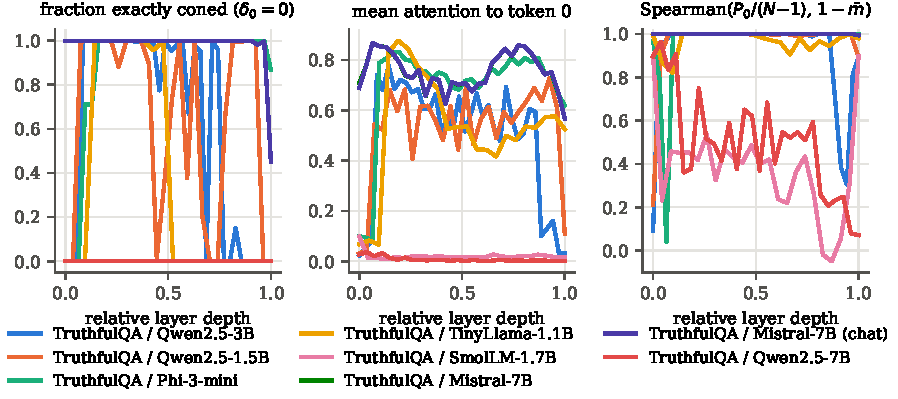
\includegraphics[width=\linewidth]{fig_sink_layers.pdf}
\caption{\textbf{Layerwise structure (TruthfulQA).} Coning (left) tracks sink attention (middle): layers with little sink attention, typically the first and last few, are rarely coned, and SmolLM-1.7B, which has no first-token sink, is never coned. Even there, $P_0$ remains rank-aligned with the star weight (right), as Theorem~\ref{thm:cone}(b) permits when $\defect_0$ is small relative to the spread of $\stw_0$.}
\label{fig:layers}
\end{figure}

\RESULTSREDUCTION

\subsection{What topology adds beyond the sink}
\label{sec:beyond}

\RESULTSBEYOND

\subsection{One-dimensional persistence}
\label{sec:onedim}

\begin{figure}[t]
\centering
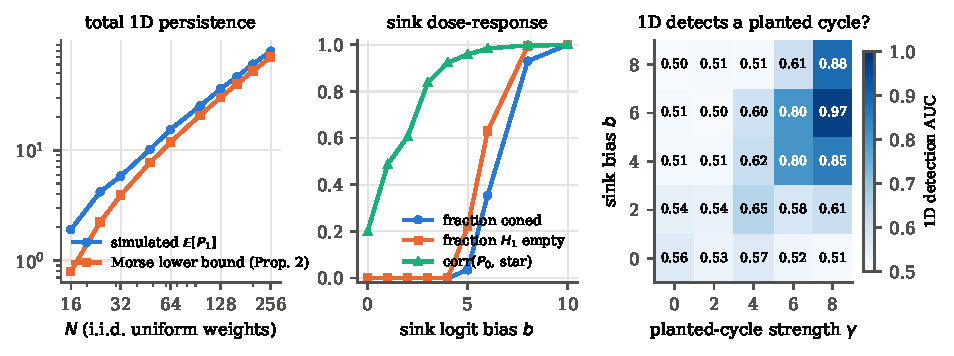
\includegraphics[width=\linewidth]{fig_sink_synthetic.pdf}
\caption{\textbf{Synthetic checks.} \emph{Left:} Proposition~\ref{prop:morse}'s lower bound against the simulated mean total $1$D persistence under i.i.d.\ weights (8 draws per $N$). \emph{Middle:} random causal attention ($N{=}40$, 200 draws per point) with a logit bias $b$ on token 0: as the sink strengthens, graphs become exactly coned, $H_1$ empties, and $P_0$ becomes a function of the star weight. \emph{Right:} AUC of $1$D total persistence for detecting a planted 6-cycle of logit strength $\gamma$ (150 draws per class). Under a strong sink ($b{=}8$) a planted cycle is invisible unless it is strong enough to break the cone.}
\label{fig:synthetic}
\end{figure}

\RESULTSONEDIM

\subsection{Hallucination detection against strong baselines}
\label{sec:detection}

\begin{table}[t]
\centering
\small
\caption{\textbf{Pooled out-of-fold ROC-AUC} (3-seed repeated grouped 10-fold CV; seed SD $\le\MaxSeedSD$). TQA: TruthfulQA; HE: HaluEval; TrQA: on-policy TriviaQA. Lex.: answer-text TF-IDF; LogP: log-probability statistics; LLM-C.: LLM-Check; Sink: $(\stw_0,\max_u D_{0u})$ per layer; 0D/1D: persistence per layer; subscript $h$: per head; Lookb.: Lookback ratios; Hidden: mid-layer probe; Non-topo.: LogP+LLM-C.+Lookb.+Hidden+row statistics. Best per row in bold; ``--'': not computed (no per-head features for HE Qwen2.5-3B). Full table in Appendix~\ref{app:tables}.}
\label{tab:auc}
\setlength{\tabcolsep}{3pt}\SinkTableAuc
\end{table}

\begin{table}[t]
\centering
\small
\caption{\textbf{Key paired comparisons} ($\Delta$AUC). ``X$-$Y'' is AUC(X)$-$AUC(Y); ``X$\mid$Y'' is AUC(Y+X)$-$AUC(Y). Defl.: sink-deflated $0$D+$1$D PH; NT: all non-topological features. $^{\equiv}$: equivalent within $\pm0.015$ (90\% interval inside the margin); $^{*}$: 95\% interval excludes $0$. Intervals and TOST power for every cell are in Appendix~\ref{app:tables}.}
\label{tab:tests}
\setlength{\tabcolsep}{4pt}\SinkTableTests
\end{table}

\begin{figure}[t]
\centering
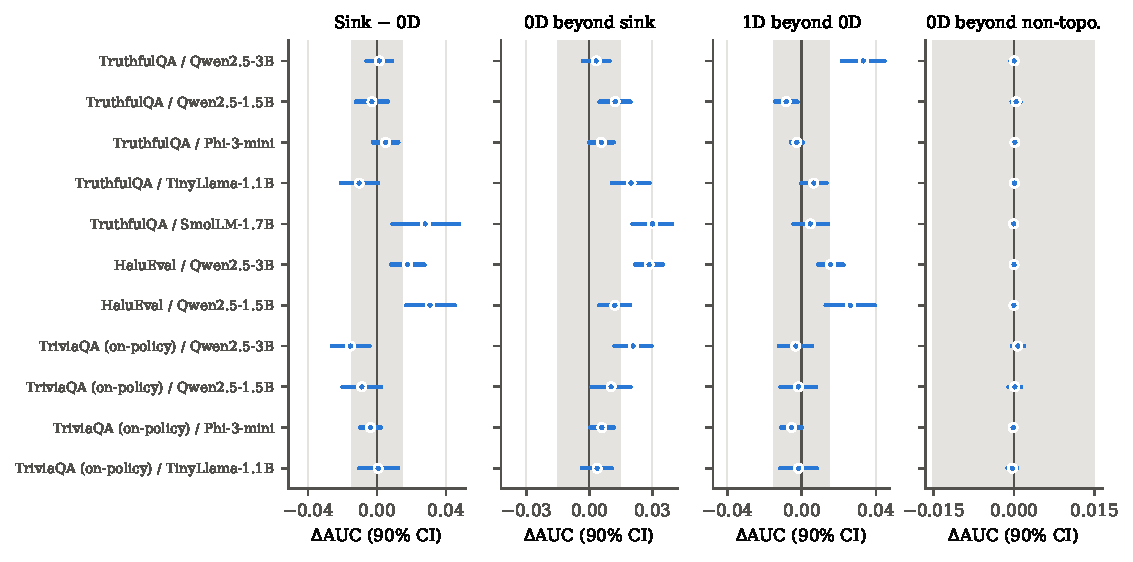
\includegraphics[width=\linewidth]{fig_sink_forest.pdf}
\caption{\textbf{Four comparisons across all settings} ($\Delta$AUC with 90\% cluster-bootstrap intervals; shaded band: $\pm0.015$). Sink features nearly reproduce $0$D; $0$D adds little beyond them; $1$D adds nothing beyond $0$D; and $0$D adds nothing beyond non-topological probes.}
\label{fig:forest}
\end{figure}

\RESULTSDETECTION

\subsection{Benchmark artifacts}
\label{sec:artifacts}

\RESULTSARTIFACTS

\section{Discussion}
\label{sec:discussion}

\RESULTSDISCUSSION

\paragraph{Limitations.} Our models range from $1.1$B to $3.8$B parameters (7B in the appendix when available); sink strength changes with scale and training \citep{gu2025attentionsink}, so the \emph{share} of coned layers is model-specific, although Theorem~\ref{thm:cone} is not. We study the head-averaged symmetrized construction and its causal directed-flag equivalent; zigzag constructions across layers \citep{samaga2026halluzig} and learned graph models \citep{charm} are outside the theorem, though their inputs are the same sink-dominated graphs. Our on-policy benchmark uses string-match grading, which mislabels some paraphrases. Teacher-forced benchmarks measure whether attention separates dataset-written true and false text, which Section~\ref{sec:artifacts} shows is partly a property of how that text was written.

\section*{Reproducibility statement}
All code is released at \url{https://anonymous.4open.science/r/ICLR-BE07/}: \texttt{sinktda/extract.py} (all features), \texttt{sinktda/evaluate.py} (every AUC, interval, and theory check), \texttt{sinktda/synthetic.py} (Figure~\ref{fig:synthetic}), and \texttt{sinktda/report.py} (every table and figure). Per-example features for all settings and the TriviaQA generations are included. Proofs are in Appendix~\ref{app:proofs}.

\section*{LLM usage statement}
LLMs were used to help implement experiment code, check reported statistics against result files, and draft and edit text. The authors verified every claim, number, proof, and citation and take full responsibility for the paper.

\bibliography{paper}
\bibliographystyle{iclr2026_conference}

\newpage
\appendix
% appendix_sink.tex -- \input by paper.tex after \appendix

\section{Proofs}
\label{app:proofs}

Throughout, $D$ is a symmetric $N\times N$ matrix with non-negative entries and zero diagonal, $K_\epsilon$ is the Vietoris--Rips complex at scale $\epsilon$, $\mathrm{filt}_D(\sigma)=\max_{u,v\in\sigma}D_{uv}$ (with $\mathrm{filt}_D(\{u\})=0$), and homology is taken over a field. Bars are half-open intervals $[b,d)$.

\subsection{Fact~\ref{fact:mst}}
All vertices enter at $0$. Processing edges in non-decreasing weight order, an edge either joins two components, in which case (elder rule) one $0$D class dies at its weight and Kruskal's algorithm adds the edge to the spanning forest, or it closes a cycle, in which case no $0$D class dies and Kruskal discards it. Hence the $N-1$ finite death times are the MST edge weights \citep{gower1969,edelsbrunner2010}.

\subsection{Theorem~\ref{thm:cone}}

\begin{lemma}[Coned filtrations]
\label{lem:coned}
If $D$ is coned at $s$, then for every $\epsilon\ge0$, $K_\epsilon=C_\epsilon\sqcup I_\epsilon$, where $C_\epsilon$ is a simplicial cone with apex $s$ and $I_\epsilon$ is a set of isolated vertices. Consequently $\tilde H_k(K_\epsilon)=0$ for every $k\ge1$.
\end{lemma}
\begin{proof}
Let $\sigma\in K_\epsilon$ with $s\notin\sigma$ and $|\sigma|\ge2$. For each $u\in\sigma$ choose $v\in\sigma\setminus\{u\}$; coning gives $D_{su}\le D_{uv}\le\mathrm{filt}_D(\sigma)\le\epsilon$. Therefore $\mathrm{filt}_D(\sigma\cup\{s\})=\mathrm{filt}_D(\sigma)$ and $\sigma\cup\{s\}\in K_\epsilon$. Now let $u\ne s$ be a vertex with $D_{su}>\epsilon$. If $u$ had an edge $\{u,v\}\in K_\epsilon$ then $D_{su}\le D_{uv}\le\epsilon$, a contradiction; so $u$ is isolated. Let $I_\epsilon$ be these vertices and $C_\epsilon$ the subcomplex on the remaining vertices. Every vertex of $C_\epsilon$ is adjacent to $s$, and by the first part every simplex of $C_\epsilon$ extends by $s$, so $C_\epsilon$ is the cone over its link of $s$ and is contractible. $H_k$ of a disjoint union is the direct sum, and isolated points have no homology in degree $\ge1$.
\end{proof}

\begin{proof}[Proof of Theorem~\ref{thm:cone}]
Fix $s$ and $\defect=\defect_s(D)$. Define $D'_{uv}=\max(D_{uv},D_{su},D_{sv})$ for $u,v\ne s$, $u\ne v$; $D'_{su}=D'_{us}=D_{su}$; $D'_{uu}=0$.

\emph{Step 1: $D\le D'\le D+\defect$ and $D'$ is coned at $s$.} The first inequality is immediate. For $u,v\ne s$, $D'_{uv}-D_{uv}=[\max(D_{su},D_{sv})-D_{uv}]_+\le\defect$. Coning: $\max(D'_{su},D'_{sv})=\max(D_{su},D_{sv})\le D'_{uv}$.

\emph{Step 2: interleaving.} Since filtration values are maxima of entries, $\mathrm{filt}_D\le\mathrm{filt}_{D'}\le\mathrm{filt}_D+\defect$. Hence for every $b$, $K_b\subseteq K'_{b+\defect}\subseteq K_{b+\defect}$, where $K'$ is the filtration of $D'$.

\emph{Step 3: (a).} The persistence map $H_k(K_b)\to H_k(K_{b+\defect})$ is induced by the composite inclusion in Step 2 and therefore factors through $H_k(K'_{b+\defect})$, which is zero for $k\ge1$ by Lemma~\ref{lem:coned}. The rank of $H_k(K_b)\to H_k(K_{b'})$ equals the number of bars $[b_i,d_i)$ with $b_i\le b$ and $d_i>b'$. A bar with $d_i-b_i>\defect$ would contribute to this rank at $b=b_i$, $b'=b_i+\defect$, a contradiction. So every bar has length at most $\defect$, and summing gives the bound on $P_k$.

\emph{Step 4: (b).} By Fact~\ref{fact:mst}, $P_0(D)=w_D(T_D)$ for an MST $T_D$ of $D$. The star $T_s=\{\{s,u\}\}_{u\ne s}$ is a spanning tree, so $P_0(D)\le w_D(T_s)=\stw_s(D)$. For the lower bound, $T_s$ is an MST of $D'$: every non-star edge $\{u,v\}$ closes the cycle $s,u,v$ in which it is a heaviest edge ($D'_{uv}\ge\max(D'_{su},D'_{sv})$), so by the cycle property it can be excluded. Hence $w_{D'}(T_{D'})=w_{D'}(T_s)=\stw_s(D)$, and
$P_0(D)=w_D(T_D)\ge w_{D'}(T_D)-(N-1)\defect\ge w_{D'}(T_{D'})-(N-1)\defect=\stw_s(D)-(N-1)\defect.$
The maximum finite $0$D death is the bottleneck value $\min_T\max_{e\in T}w(e)$, which is attained by any MST; it is at most $\max_u D_{su}$ (the star is a spanning tree) and is $1$-Lipschitz in the sup-norm, which gives the lower bound because the bottleneck of $D'$ is $\max_u D_{su}$.

\emph{Step 5: (c).} If $\defect=0$ then $D'=D$, and the claims follow from Lemma~\ref{lem:coned} and Step 4.
\end{proof}

\begin{proof}[Proof of Corollary~\ref{cor:causal}]
For $u>v$, $A_{vu}=0$, so $D_{uv}=1-A_{uv}$; in particular $D_{0u}=1-A_{u0}$. For $1\le v<u$, $\max(D_{0u},D_{0v})-D_{uv}=A_{uv}-\min(A_{u0},A_{v0})$. Substitute into Theorem~\ref{thm:cone}.
\end{proof}

\subsection{Proposition~\ref{prop:morse}}
\begin{proof}
With i.i.d.\ uniform weights, the edges with $D_{uv}\le p$ form an Erd\H{o}s--R\'enyi graph $G(N,p)$ and $K_p$ is its clique (flag) complex. Every $1$D bar is contained in $[0,1)$, because $K_1$ is the full simplex. Writing $\beta_1(p)$ for the first Betti number of $K_p$, the number of bars alive at $p$ is $\beta_1(p)$, so $P_1=\int_0^1\beta_1(p)\,dp$.
For any finite complex with $f_i$ faces of dimension $i$, the strong Morse inequality at degree $2$ reads $\beta_2-\beta_1+\beta_0\le f_2-f_1+f_0$ \citep{edelsbrunner2010}, hence $\beta_1\ge f_1-f_0-f_2+\beta_0+\beta_2\ge f_1-f_0-f_2$. Since also $\beta_1\ge0$, Jensen's inequality gives $\mathbb{E}\beta_1(p)\ge[\mathbb{E}f_1-f_0-\mathbb{E}f_2]_+=[\binom N2p-N-\binom N3p^3]_+$. Integrating over $p$ gives the first inequality. With $p=x/\sqrt N$ the integrand is $N^{3/2}(x/2-x^3/6)-N+O(N^{1/2})$, positive on $x\in(2/\sqrt N\cdot(1+o(1)),\sqrt3)$, and
$\int_0^1[\cdot]_+dp=N\int_0^{\sqrt3}\big(\tfrac x2-\tfrac{x^3}{6}\big)dx-O(\sqrt N)=\tfrac38N-O(\sqrt N).$
For the upper bound, $\beta_1\le f_1$ gives $\mathbb{E}P_1\le\int_0^1\binom N2p\,dp=\binom N2/2$.
\end{proof}
Numerically, the integral equals $0.79, 3.92, 11.9, 30.2, 70.1$ at $N=16,32,64,128,256$, against simulated means $1.84, 6.46, 22.4, 64.9, 168.0$ (Figure~\ref{fig:synthetic}, left). Both grow super-linearly over this range (log-log slopes $1.55$ and $1.61$); the lower bound's slope tends to $1$ as $N\to\infty$.

\subsection{Directed flag complexes on causal attention}
\label{app:directed}
\begin{theorem}[Directed flag collapse]
\label{thm:directed}
Let $A$ be lower-triangular with $A_{ij}>0$ for all $j\le i$ (the diagonal included; self-loops are ignored). Let $\mathrm{DFl}(A)$ be the filtered directed flag complex \citep{flagser2020} of the digraph with an edge $i\to j$ for every $j<i$ and weight $1-A_{ij}$, and let $\VR(D)$ be as above with $D=1-\max(A,A^\top)$. Then $\mathrm{DFl}(A)$ and $\VR(D)$ are isomorphic filtered complexes, so $\dgm_k(\mathrm{DFl}(A))=\dgm_k(\VR(D))$ for all $k$. The same holds for any weighting $w(i\to j)=\phi(A_{ij})$ with $D_{ij}=\phi(\max(A_{ij},A_{ji}))$ and $\phi$ non-increasing.
\end{theorem}
\begin{proof}
A directed $k$-simplex is an ordered tuple $(v_0,\dots,v_k)$ with an edge $v_a\to v_b$ for all $a<b$. Edges exist only from later to earlier tokens, so a vertex set $S$ supports exactly one directed simplex, its elements in decreasing order; every other ordering uses a missing forward edge. (A missing edge is not a zero-weight edge; encoding it as weight $0$ would admit all orderings, a common implementation error.) This bijection preserves faces. Its filtration value is $\max_{a<b}(1-A_{v_av_b})$, and for $u>v$, $D_{uv}=1-A_{uv}$, so the undirected value $\max_{u,v\in S}D_{uv}$ is the same number.
\end{proof}
We verified the bijection and the filtration identity by explicit enumeration on $420$ random causal matrices ($N\le8$, four families including tie-dense and underflowing matrices; $30{,}060$ vertex sets; zero violations), and confirmed that the identity fails for bidirectional attention, where a set of size $n$ supports $n!$ orderings. The collapse is a consequence of causality, so directional treatments that are well motivated for bidirectional encoders \citep{kushnareva2021} do not transfer to decoders.

\section{Implementation and protocol details}
\label{app:impl}

\paragraph{Extraction.} Models run in float16 on Apple-silicon (MPS) with eager attention. For each example we run one forward pass with attentions and hidden states, average heads, and form $D$ in float64. Ripser \citep{bauer2021ripser} computes $0$D/$1$D barcodes; per-head MSTs use a batched dense Prim's algorithm (SciPy's sparse MST drops explicit zero-weight edges, which occur when $A_{u0}\approx1$). $\defect_0$ uses the closed form of Corollary~\ref{cor:causal}; $\min_s\defect_s$ is computed by brute force over all apexes. \textsc{Deflated} deletes token 0 and renormalizes each row over the remaining causal support. \textsc{Answer-only} restricts $D$ to the answer tokens without renormalization. The Lookback ratio of head $h$ is the mean over answer tokens $t$ of $\bar a_{\mathrm{ctx}}/(\bar a_{\mathrm{ctx}}+\bar a_{\mathrm{new}})$, with $\bar a$ the mean attention from $t$ to prompt tokens and to answer tokens up to $t$. The LLM-Check score of a head is the mean log diagonal attention (the log-determinant of the triangular attention kernel divided by $N$), summed over heads per layer. Log-probability features are the mean, minimum, and sum of answer-token log-probabilities, mean and maximum predictive entropy, and mean maximum softmax probability. Hidden states are mean-pooled over answer tokens at layer $\lfloor L/2\rfloor$.

\paragraph{Prompts.} TruthfulQA uses each model's native format: the Qwen chat template with the default system turn, \texttt{<|user|>\ldots<|end|>} for Phi-3, \texttt{<|user|>\ldots</s>} for TinyLlama, ChatML without system turn for SmolLM, and \texttt{[INST]\ldots[/INST]} for Mistral. HaluEval uses \texttt{Knowledge: \ldots\textbackslash nQuestion: \ldots\textbackslash nAnswer: }. The on-policy prompt is the model's chat template around ``Answer the following question with a short phrase only, no explanation. Question: \ldots''. Token 0 is whatever token the format places first (BOS for TinyLlama and Mistral, \texttt{<|user|>} for Phi-3, whose tokenizer adds no BOS, \texttt{<|im\_start|>} for Qwen and SmolLM, and ``Knowledge'' for Qwen on HaluEval); the theorem does not require it to be a special token.

\paragraph{On-policy benchmark.}
\begin{table}[h]
\centering
\small
\caption{\textbf{TriviaQA on-policy benchmark.} $2{,}000$ validation questions sampled with seed 0; greedy decoding, first line of the answer, at most 24 new tokens. An answer is correct if any normalized gold alias (lower-cased, punctuation and articles removed) occurs in the normalized answer as a whole-word span. Empty answers are dropped.}
\label{tab:onpolicy}
\SinkTableOnpolicy
\end{table}

\paragraph{Statistics.} Bootstrap resamples are drawn over questions (both rows of a pair move together). TOST power at margin $\epsilon$ assumes a true difference of $0$ and a normal sampling distribution with the bootstrap SE: $2\Phi(\epsilon/\mathrm{SE}-z_{0.95})-1$. Repeated-CV predictions are averaged before bootstrapping, so the intervals reflect sampling of questions for a fixed, split-averaged predictor; the seed-to-seed SD of the pooled AUC is reported separately and is below $0.004$ everywhere.

\section{Full results}
\label{app:tables}
\small
\begin{longtable}{llrrrr}
\toprule
Setting & Bank & dim & AUC & seed SD & pair acc. \\
\midrule\endhead
TQA Qw3B & NONTOPO+DEFL & 2954 & 0.928 & 0.0007 & 0.931 \\
TQA Qw3B & 0D & 72 & 0.754 & 0.0017 & 0.799 \\
TQA Qw3B & SINK & 72 & 0.740 & 0.0028 & 0.765 \\
TQA Qw3B & 1D & 144 & 0.602 & 0.0018 & 0.583 \\
TQA Qw3B & DEFL & 216 & 0.717 & 0.0009 & 0.748 \\
TQA Qw3B & ANS & 216 & 0.752 & 0.0017 & 0.745 \\
TQA Qw3B & ROWSTAT & 72 & 0.751 & 0.0003 & 0.829 \\
TQA Qw3B & LOGPROB & 6 & 0.631 & 0.0008 & 0.682 \\
TQA Qw3B & HIDDEN & 2048 & 0.913 & 0.0008 & 0.916 \\
TQA Qw3B & LEX & -- & 0.820 & 0.0014 & 0.829 \\
TQA Qw3B & LEGACY MSTPROXY & 36 & 0.714 & 0.0006 & 0.786 \\
TQA Qw3B & LLMCHECK & 36 & 0.693 & 0.0011 & 0.764 \\
TQA Qw3B & LOOKBACK & 576 & 0.897 & 0.0026 & 0.906 \\
TQA Qw3B & PH 0D & 1152 & 0.854 & 0.0022 & 0.857 \\
TQA Qw3B & PH 0DTOT & 576 & 0.844 & 0.0010 & 0.868 \\
TQA Qw3B & PH SINK & 576 & 0.850 & 0.0018 & 0.865 \\
TQA Qw3B & PH ENT & 576 & 0.859 & 0.0016 & 0.906 \\
TQA Qw3B & 0D+SINK & 144 & 0.757 & 0.0019 & 0.788 \\
TQA Qw3B & 0D+1D & 216 & 0.760 & 0.0012 & 0.789 \\
TQA Qw3B & SINK+DEFL & 288 & 0.772 & 0.0032 & 0.802 \\
TQA Qw3B & SINK+ANS & 288 & 0.784 & 0.0026 & 0.791 \\
TQA Qw3B & LEX+DEFL & -- & 0.829 & 0.0010 & 0.842 \\
TQA Qw3B & LEX+SINK & -- & 0.843 & 0.0021 & 0.859 \\
TQA Qw3B & LEX+0D & -- & 0.847 & 0.0016 & 0.860 \\
TQA Qw3B & HIDDEN+0D & 2120 & 0.914 & 0.0009 & 0.917 \\
TQA Qw3B & LOGPROB+0D & 78 & 0.787 & 0.0022 & 0.820 \\
TQA Qw3B & SINK+1D & 216 & 0.747 & 0.0021 & 0.767 \\
TQA Qw3B & NONTOPO+0D & 2810 & 0.928 & 0.0004 & 0.936 \\
TQA Qw3B & LEN & 2 & 0.529 & 0.0003 & 0.567 \\
TQA Qw3B & NONTOPO & 2738 & 0.927 & 0.0006 & 0.938 \\
TQA Qw3B & PH SINK+PH 0DTOT & 1152 & 0.860 & 0.0032 & 0.889 \\
TQA Qw1.5B & 0D & 56 & 0.726 & 0.0007 & 0.767 \\
TQA Qw1.5B & LEN & 2 & 0.529 & 0.0003 & 0.567 \\
TQA Qw1.5B & LEX+SINK & -- & 0.833 & 0.0008 & 0.846 \\
TQA Qw1.5B & LEX+0D & -- & 0.835 & 0.0017 & 0.841 \\
TQA Qw1.5B & HIDDEN+0D & 1592 & 0.916 & 0.0014 & 0.924 \\
TQA Qw1.5B & LOGPROB+0D & 62 & 0.740 & 0.0013 & 0.797 \\
TQA Qw1.5B & NONTOPO+DEFL & 2130 & 0.917 & 0.0014 & 0.923 \\
TQA Qw1.5B & NONTOPO+0D & 2018 & 0.917 & 0.0014 & 0.927 \\
TQA Qw1.5B & NONTOPO & 1962 & 0.917 & 0.0013 & 0.928 \\
TQA Qw1.5B & PH SINK+PH 0DTOT & 672 & 0.841 & 0.0013 & 0.867 \\
TQA Qw1.5B & SINK+1D & 168 & 0.715 & 0.0017 & 0.769 \\
TQA Qw1.5B & SINK+ANS & 224 & 0.761 & 0.0027 & 0.753 \\
TQA Qw1.5B & SINK+DEFL & 224 & 0.757 & 0.0028 & 0.802 \\
TQA Qw1.5B & 0D+1D & 168 & 0.718 & 0.0013 & 0.767 \\
TQA Qw1.5B & 0D+SINK & 112 & 0.735 & 0.0012 & 0.766 \\
TQA Qw1.5B & LEX+DEFL & -- & 0.825 & 0.0019 & 0.836 \\
TQA Qw1.5B & PH SINK & 336 & 0.830 & 0.0008 & 0.851 \\
TQA Qw1.5B & PH ENT & 336 & 0.833 & 0.0025 & 0.852 \\
TQA Qw1.5B & 1D & 112 & 0.586 & 0.0014 & 0.644 \\
TQA Qw1.5B & DEFL & 168 & 0.703 & 0.0042 & 0.755 \\
TQA Qw1.5B & ANS & 168 & 0.697 & 0.0040 & 0.700 \\
TQA Qw1.5B & ROWSTAT & 56 & 0.738 & 0.0014 & 0.815 \\
TQA Qw1.5B & LOGPROB & 6 & 0.638 & 0.0007 & 0.682 \\
TQA Qw1.5B & SINK & 56 & 0.723 & 0.0019 & 0.771 \\
TQA Qw1.5B & LEX & -- & 0.820 & 0.0014 & 0.829 \\
TQA Qw1.5B & LEGACY MSTPROXY & 28 & 0.698 & 0.0010 & 0.786 \\
TQA Qw1.5B & LLMCHECK & 28 & 0.666 & 0.0005 & 0.743 \\
TQA Qw1.5B & LOOKBACK & 336 & 0.851 & 0.0020 & 0.856 \\
TQA Qw1.5B & PH 0D & 672 & 0.838 & 0.0012 & 0.847 \\
TQA Qw1.5B & HIDDEN & 1536 & 0.916 & 0.0012 & 0.923 \\
TQA Qw1.5B & PH 0DTOT & 336 & 0.819 & 0.0011 & 0.838 \\
TQA Phi-3 & LOOKBACK & 1024 & 0.892 & 0.0004 & 0.903 \\
TQA Phi-3 & LLMCHECK & 32 & 0.653 & 0.0007 & 0.754 \\
TQA Phi-3 & LEGACY MSTPROXY & 32 & 0.614 & 0.0008 & 0.695 \\
TQA Phi-3 & LEX & -- & 0.820 & 0.0014 & 0.829 \\
TQA Phi-3 & HIDDEN & 3072 & 0.933 & 0.0007 & 0.947 \\
TQA Phi-3 & ANS & 192 & 0.623 & 0.0048 & 0.655 \\
TQA Phi-3 & ROWSTAT & 64 & 0.661 & 0.0011 & 0.734 \\
TQA Phi-3 & DEFL & 192 & 0.639 & 0.0011 & 0.685 \\
TQA Phi-3 & 1D & 128 & 0.529 & 0.0021 & 0.551 \\
TQA Phi-3 & SINK & 64 & 0.652 & 0.0007 & 0.707 \\
TQA Phi-3 & PH 0D & 2048 & 0.868 & 0.0006 & 0.879 \\
TQA Phi-3 & LOGPROB & 6 & 0.578 & 0.0017 & 0.599 \\
TQA Phi-3 & PH 0DTOT & 1024 & 0.846 & 0.0020 & 0.884 \\
TQA Phi-3 & LEX+DEFL & -- & 0.802 & 0.0010 & 0.827 \\
TQA Phi-3 & PH ENT & 1024 & 0.864 & 0.0011 & 0.897 \\
TQA Phi-3 & 0D+SINK & 128 & 0.658 & 0.0007 & 0.707 \\
TQA Phi-3 & 0D+1D & 192 & 0.645 & 0.0012 & 0.707 \\
TQA Phi-3 & SINK+DEFL & 256 & 0.685 & 0.0015 & 0.727 \\
TQA Phi-3 & SINK+ANS & 256 & 0.672 & 0.0013 & 0.709 \\
TQA Phi-3 & SINK+1D & 192 & 0.654 & 0.0010 & 0.705 \\
TQA Phi-3 & NONTOPO & 4198 & 0.936 & 0.0006 & 0.941 \\
TQA Phi-3 & NONTOPO+0D & 4262 & 0.936 & 0.0006 & 0.944 \\
TQA Phi-3 & NONTOPO+DEFL & 4390 & 0.937 & 0.0007 & 0.942 \\
TQA Phi-3 & LOGPROB+0D & 70 & 0.656 & 0.0010 & 0.699 \\
TQA Phi-3 & HIDDEN+0D & 3136 & 0.933 & 0.0008 & 0.944 \\
TQA Phi-3 & LEX+0D & -- & 0.821 & 0.0003 & 0.842 \\
TQA Phi-3 & LEX+SINK & -- & 0.820 & 0.0005 & 0.832 \\
TQA Phi-3 & PH SINK & 1024 & 0.871 & 0.0008 & 0.898 \\
TQA Phi-3 & PH SINK+PH 0DTOT & 2048 & 0.871 & 0.0007 & 0.906 \\
TQA Phi-3 & LEN & 2 & 0.522 & 0.0004 & 0.562 \\
TQA Phi-3 & 0D & 64 & 0.647 & 0.0010 & 0.717 \\
TQA TinyLl. & LEN & 2 & 0.523 & 0.0005 & 0.556 \\
TQA TinyLl. & 0D & 44 & 0.654 & 0.0012 & 0.727 \\
TQA TinyLl. & SINK & 44 & 0.644 & 0.0008 & 0.720 \\
TQA TinyLl. & 1D & 88 & 0.593 & 0.0010 & 0.677 \\
TQA TinyLl. & DEFL & 132 & 0.652 & 0.0028 & 0.704 \\
TQA TinyLl. & ANS & 132 & 0.646 & 0.0041 & 0.683 \\
TQA TinyLl. & ROWSTAT & 44 & 0.660 & 0.0016 & 0.744 \\
TQA TinyLl. & LOGPROB & 6 & 0.637 & 0.0010 & 0.646 \\
TQA TinyLl. & HIDDEN & 2048 & 0.883 & 0.0013 & 0.879 \\
TQA TinyLl. & LEX & -- & 0.820 & 0.0014 & 0.829 \\
TQA TinyLl. & LEGACY MSTPROXY & 22 & 0.627 & 0.0008 & 0.738 \\
TQA TinyLl. & LLMCHECK & 22 & 0.614 & 0.0007 & 0.701 \\
TQA TinyLl. & LOOKBACK & 704 & 0.850 & 0.0028 & 0.846 \\
TQA TinyLl. & PH 0D & 1408 & 0.805 & 0.0022 & 0.821 \\
TQA TinyLl. & LEX+DEFL & -- & 0.824 & 0.0011 & 0.837 \\
TQA TinyLl. & PH SINK+PH 0DTOT & 1408 & 0.811 & 0.0027 & 0.840 \\
TQA TinyLl. & LEX+0D & -- & 0.829 & 0.0011 & 0.837 \\
TQA TinyLl. & HIDDEN+0D & 2092 & 0.883 & 0.0014 & 0.879 \\
TQA TinyLl. & LOGPROB+0D & 50 & 0.682 & 0.0010 & 0.717 \\
TQA TinyLl. & NONTOPO+DEFL & 2956 & 0.884 & 0.0009 & 0.882 \\
TQA TinyLl. & NONTOPO+0D & 2868 & 0.885 & 0.0012 & 0.887 \\
TQA TinyLl. & NONTOPO & 2824 & 0.885 & 0.0011 & 0.887 \\
TQA TinyLl. & PH SINK & 704 & 0.807 & 0.0025 & 0.845 \\
TQA TinyLl. & PH 0DTOT & 704 & 0.804 & 0.0018 & 0.831 \\
TQA TinyLl. & LEX+SINK & -- & 0.831 & 0.0012 & 0.832 \\
TQA TinyLl. & SINK+ANS & 176 & 0.687 & 0.0033 & 0.722 \\
TQA TinyLl. & SINK+DEFL & 176 & 0.689 & 0.0015 & 0.750 \\
TQA TinyLl. & 0D+1D & 132 & 0.659 & 0.0017 & 0.734 \\
TQA TinyLl. & 0D+SINK & 88 & 0.663 & 0.0004 & 0.723 \\
TQA TinyLl. & PH ENT & 704 & 0.817 & 0.0009 & 0.838 \\
TQA TinyLl. & SINK+1D & 132 & 0.651 & 0.0023 & 0.741 \\
TQA SmolLM & LEX+DEFL & -- & 0.822 & 0.0005 & 0.842 \\
TQA SmolLM & LEN & 2 & 0.524 & 0.0003 & 0.554 \\
TQA SmolLM & NONTOPO+0D & 2942 & 0.899 & 0.0012 & 0.902 \\
TQA SmolLM & PH SINK+PH 0DTOT & 1536 & 0.825 & 0.0021 & 0.856 \\
TQA SmolLM & NONTOPO & 2894 & 0.899 & 0.0015 & 0.903 \\
TQA SmolLM & SINK+DEFL & 192 & 0.652 & 0.0027 & 0.674 \\
TQA SmolLM & NONTOPO+DEFL & 3038 & 0.899 & 0.0011 & 0.897 \\
TQA SmolLM & LOGPROB+0D & 54 & 0.614 & 0.0011 & 0.628 \\
TQA SmolLM & HIDDEN+0D & 2096 & 0.894 & 0.0021 & 0.891 \\
TQA SmolLM & LEX+0D & -- & 0.827 & 0.0009 & 0.840 \\
TQA SmolLM & LEX+SINK & -- & 0.819 & 0.0015 & 0.825 \\
TQA SmolLM & 0D+1D & 144 & 0.588 & 0.0018 & 0.646 \\
TQA SmolLM & 0D+SINK & 96 & 0.641 & 0.0027 & 0.670 \\
TQA SmolLM & PH ENT & 768 & 0.834 & 0.0007 & 0.843 \\
TQA SmolLM & PH SINK & 768 & 0.720 & 0.0009 & 0.776 \\
TQA SmolLM & SINK+1D & 144 & 0.632 & 0.0028 & 0.645 \\
TQA SmolLM & PH 0DTOT & 768 & 0.819 & 0.0018 & 0.846 \\
TQA SmolLM & LOOKBACK & 768 & 0.863 & 0.0017 & 0.865 \\
TQA SmolLM & LLMCHECK & 24 & 0.604 & 0.0006 & 0.685 \\
TQA SmolLM & LEGACY MSTPROXY & 24 & 0.585 & 0.0011 & 0.681 \\
TQA SmolLM & LEX & -- & 0.820 & 0.0014 & 0.829 \\
TQA SmolLM & HIDDEN & 2048 & 0.894 & 0.0022 & 0.891 \\
TQA SmolLM & LOGPROB & 6 & 0.589 & 0.0010 & 0.591 \\
TQA SmolLM & ROWSTAT & 48 & 0.673 & 0.0013 & 0.742 \\
TQA SmolLM & ANS & 144 & 0.629 & 0.0034 & 0.634 \\
TQA SmolLM & DEFL & 144 & 0.592 & 0.0024 & 0.656 \\
TQA SmolLM & 1D & 96 & 0.545 & 0.0006 & 0.569 \\
TQA SmolLM & SINK & 48 & 0.611 & 0.0020 & 0.632 \\
TQA SmolLM & 0D & 48 & 0.584 & 0.0028 & 0.655 \\
TQA SmolLM & PH 0D & 1536 & 0.798 & 0.0011 & 0.820 \\
TQA SmolLM & SINK+ANS & 192 & 0.646 & 0.0024 & 0.655 \\
HE Qw3B & LOGPROB+0D & 78 & 0.993 & 0.0003 & 0.990 \\
HE Qw3B & LEX+DEFL & -- & 0.970 & 0.0005 & 0.977 \\
HE Qw3B & SINK+1D & 216 & 0.842 & 0.0004 & 0.938 \\
HE Qw3B & SINK+ANS & 288 & 0.978 & 0.0007 & 0.977 \\
HE Qw3B & SINK+DEFL & 288 & 0.882 & 0.0026 & 0.961 \\
HE Qw3B & 0D+1D & 216 & 0.830 & 0.0023 & 0.944 \\
HE Qw3B & 0D+SINK & 144 & 0.858 & 0.0009 & 0.946 \\
HE Qw3B & LEGACY MSTPROXY & 36 & 0.733 & 0.0001 & 0.960 \\
HE Qw3B & LEX+0D & -- & 0.979 & 0.0001 & 0.983 \\
HE Qw3B & HIDDEN & 2048 & 0.999 & 0.0000 & 0.999 \\
HE Qw3B & LOGPROB & 6 & 0.993 & 0.0003 & 0.986 \\
HE Qw3B & ROWSTAT & 72 & 0.830 & 0.0003 & 0.975 \\
HE Qw3B & ANS & 216 & 0.974 & 0.0008 & 0.974 \\
HE Qw3B & DEFL & 216 & 0.832 & 0.0001 & 0.958 \\
HE Qw3B & 1D & 144 & 0.709 & 0.0010 & 0.892 \\
HE Qw3B & SINK & 72 & 0.827 & 0.0008 & 0.930 \\
HE Qw3B & 0D & 72 & 0.816 & 0.0009 & 0.929 \\
HE Qw3B & LEN & 2 & 0.962 & 0.0001 & 0.970 \\
HE Qw3B & LEX+SINK & -- & 0.980 & 0.0002 & 0.983 \\
HE Qw3B & HIDDEN+0D & 2120 & 0.999 & 0.0001 & 0.999 \\
HE Qw3B & LEX & -- & 0.981 & 0.0004 & 0.977 \\
HE Qw1.5B & LEN & 2 & 0.967 & 0.0002 & 0.976 \\
HE Qw1.5B & LEX+DEFL & -- & 0.956 & 0.0002 & 0.986 \\
HE Qw1.5B & LEX+0D & -- & 0.971 & 0.0004 & 0.986 \\
HE Qw1.5B & HIDDEN+0D & 1592 & 0.999 & 0.0001 & 1.000 \\
HE Qw1.5B & LOGPROB+0D & 62 & 0.993 & 0.0004 & 0.994 \\
HE Qw1.5B & NONTOPO+DEFL & 2130 & 0.999 & 0.0004 & 1.000 \\
HE Qw1.5B & NONTOPO+0D & 2018 & 0.999 & 0.0001 & 1.000 \\
HE Qw1.5B & NONTOPO & 1962 & 0.999 & 0.0003 & 1.000 \\
HE Qw1.5B & PH SINK+PH 0DTOT & 672 & 0.931 & 0.0024 & 0.998 \\
HE Qw1.5B & SINK+1D & 168 & 0.826 & 0.0035 & 0.940 \\
HE Qw1.5B & SINK+ANS & 224 & 0.970 & 0.0022 & 0.990 \\
HE Qw1.5B & SINK+DEFL & 224 & 0.872 & 0.0028 & 0.962 \\
HE Qw1.5B & 0D+1D & 168 & 0.815 & 0.0032 & 0.922 \\
HE Qw1.5B & 0D+SINK & 112 & 0.832 & 0.0015 & 0.924 \\
HE Qw1.5B & PH ENT & 336 & 0.933 & 0.0011 & 0.996 \\
HE Qw1.5B & PH SINK & 336 & 0.922 & 0.0007 & 0.998 \\
HE Qw1.5B & LEX+SINK & -- & 0.968 & 0.0005 & 0.984 \\
HE Qw1.5B & PH 0D & 672 & 0.949 & 0.0027 & 0.974 \\
HE Qw1.5B & 0D & 56 & 0.789 & 0.0014 & 0.918 \\
HE Qw1.5B & SINK & 56 & 0.820 & 0.0015 & 0.934 \\
HE Qw1.5B & 1D & 112 & 0.747 & 0.0006 & 0.878 \\
HE Qw1.5B & DEFL & 168 & 0.825 & 0.0021 & 0.952 \\
HE Qw1.5B & ANS & 168 & 0.969 & 0.0010 & 0.983 \\
HE Qw1.5B & ROWSTAT & 56 & 0.788 & 0.0017 & 0.984 \\
HE Qw1.5B & PH 0DTOT & 336 & 0.921 & 0.0007 & 0.996 \\
HE Qw1.5B & HIDDEN & 1536 & 0.999 & 0.0001 & 1.000 \\
HE Qw1.5B & LEX & -- & 0.979 & 0.0004 & 0.980 \\
HE Qw1.5B & LEGACY MSTPROXY & 28 & 0.719 & 0.0003 & 0.976 \\
HE Qw1.5B & LLMCHECK & 28 & 0.791 & 0.0005 & 0.978 \\
HE Qw1.5B & LOOKBACK & 336 & 0.997 & 0.0001 & 0.996 \\
HE Qw1.5B & LOGPROB & 6 & 0.993 & 0.0001 & 0.992 \\
TrQA Qw3B & LOOKBACK & 576 & 0.861 & 0.0013 & -- \\
TrQA Qw3B & LLMCHECK & 36 & 0.688 & 0.0012 & -- \\
TrQA Qw3B & LEGACY MSTPROXY & 36 & 0.691 & 0.0033 & -- \\
TrQA Qw3B & LEX & -- & 0.596 & 0.0039 & -- \\
TrQA Qw3B & HIDDEN & 2048 & 0.841 & 0.0042 & -- \\
TrQA Qw3B & LOGPROB & 6 & 0.839 & 0.0002 & -- \\
TrQA Qw3B & DEFL & 216 & 0.684 & 0.0043 & -- \\
TrQA Qw3B & ANS & 216 & 0.719 & 0.0020 & -- \\
TrQA Qw3B & 1D & 144 & 0.601 & 0.0031 & -- \\
TrQA Qw3B & SINK & 72 & 0.717 & 0.0038 & -- \\
TrQA Qw3B & 0D & 72 & 0.732 & 0.0038 & -- \\
TrQA Qw3B & PH 0D & 1152 & 0.807 & 0.0017 & -- \\
TrQA Qw3B & ROWSTAT & 72 & 0.724 & 0.0046 & -- \\
TrQA Qw3B & LEN & 2 & 0.569 & 0.0014 & -- \\
TrQA Qw3B & PH 0DTOT & 576 & 0.807 & 0.0012 & -- \\
TrQA Qw3B & PH ENT & 576 & 0.810 & 0.0007 & -- \\
TrQA Qw3B & PH SINK & 576 & 0.820 & 0.0021 & -- \\
TrQA Qw3B & LEX+SINK & -- & 0.724 & 0.0005 & -- \\
TrQA Qw3B & LEX+0D & -- & 0.733 & 0.0011 & -- \\
TrQA Qw3B & HIDDEN+0D & 2120 & 0.843 & 0.0040 & -- \\
TrQA Qw3B & LOGPROB+0D & 78 & 0.843 & 0.0022 & -- \\
TrQA Qw3B & NONTOPO+DEFL & 2954 & 0.870 & 0.0029 & -- \\
TrQA Qw3B & NONTOPO+0D & 2810 & 0.870 & 0.0027 & -- \\
TrQA Qw3B & LEX+DEFL & -- & 0.690 & 0.0031 & -- \\
TrQA Qw3B & PH SINK+PH 0DTOT & 1152 & 0.824 & 0.0017 & -- \\
TrQA Qw3B & SINK+1D & 216 & 0.718 & 0.0035 & -- \\
TrQA Qw3B & SINK+ANS & 288 & 0.752 & 0.0010 & -- \\
TrQA Qw3B & SINK+DEFL & 288 & 0.719 & 0.0038 & -- \\
TrQA Qw3B & 0D+1D & 216 & 0.729 & 0.0022 & -- \\
TrQA Qw3B & 0D+SINK & 144 & 0.738 & 0.0050 & -- \\
TrQA Qw3B & NONTOPO & 2738 & 0.870 & 0.0028 & -- \\
TrQA Qw1.5B & LOOKBACK & 336 & 0.824 & 0.0017 & -- \\
TrQA Qw1.5B & LLMCHECK & 28 & 0.676 & 0.0029 & -- \\
TrQA Qw1.5B & LEGACY MSTPROXY & 28 & 0.685 & 0.0014 & -- \\
TrQA Qw1.5B & LEX & -- & 0.609 & 0.0033 & -- \\
TrQA Qw1.5B & HIDDEN & 1536 & 0.855 & 0.0031 & -- \\
TrQA Qw1.5B & LOGPROB & 6 & 0.823 & 0.0006 & -- \\
TrQA Qw1.5B & PH 0D & 672 & 0.768 & 0.0013 & -- \\
TrQA Qw1.5B & ANS & 168 & 0.675 & 0.0035 & -- \\
TrQA Qw1.5B & 1D & 112 & 0.574 & 0.0024 & -- \\
TrQA Qw1.5B & SINK & 56 & 0.707 & 0.0000 & -- \\
TrQA Qw1.5B & 0D & 56 & 0.716 & 0.0004 & -- \\
TrQA Qw1.5B & LEN & 2 & 0.588 & 0.0012 & -- \\
TrQA Qw1.5B & ROWSTAT & 56 & 0.720 & 0.0008 & -- \\
TrQA Qw1.5B & DEFL & 168 & 0.655 & 0.0016 & -- \\
TrQA Qw1.5B & PH 0DTOT & 336 & 0.759 & 0.0051 & -- \\
TrQA Qw1.5B & PH ENT & 336 & 0.768 & 0.0025 & -- \\
TrQA Qw1.5B & PH SINK & 336 & 0.767 & 0.0034 & -- \\
TrQA Qw1.5B & LEX+DEFL & -- & 0.672 & 0.0047 & -- \\
TrQA Qw1.5B & LEX+0D & -- & 0.721 & 0.0031 & -- \\
TrQA Qw1.5B & HIDDEN+0D & 1592 & 0.855 & 0.0032 & -- \\
TrQA Qw1.5B & LOGPROB+0D & 62 & 0.828 & 0.0007 & -- \\
TrQA Qw1.5B & NONTOPO+DEFL & 2130 & 0.872 & 0.0024 & -- \\
TrQA Qw1.5B & NONTOPO+0D & 2018 & 0.873 & 0.0025 & -- \\
TrQA Qw1.5B & LEX+SINK & -- & 0.715 & 0.0036 & -- \\
TrQA Qw1.5B & PH SINK+PH 0DTOT & 672 & 0.772 & 0.0022 & -- \\
TrQA Qw1.5B & SINK+1D & 168 & 0.709 & 0.0028 & -- \\
TrQA Qw1.5B & SINK+ANS & 224 & 0.726 & 0.0059 & -- \\
TrQA Qw1.5B & SINK+DEFL & 224 & 0.719 & 0.0023 & -- \\
TrQA Qw1.5B & NONTOPO & 1962 & 0.873 & 0.0023 & -- \\
TrQA Qw1.5B & 0D+1D & 168 & 0.714 & 0.0015 & -- \\
TrQA Qw1.5B & 0D+SINK & 112 & 0.717 & 0.0006 & -- \\
TrQA Phi-3 & LOOKBACK & 1024 & 0.840 & 0.0016 & -- \\
TrQA Phi-3 & LLMCHECK & 32 & 0.676 & 0.0018 & -- \\
TrQA Phi-3 & LEGACY MSTPROXY & 32 & 0.669 & 0.0002 & -- \\
TrQA Phi-3 & LEX & -- & 0.635 & 0.0083 & -- \\
TrQA Phi-3 & HIDDEN & 3072 & 0.867 & 0.0035 & -- \\
TrQA Phi-3 & ROWSTAT & 64 & 0.728 & 0.0006 & -- \\
TrQA Phi-3 & PH 0D & 2048 & 0.807 & 0.0024 & -- \\
TrQA Phi-3 & ANS & 192 & 0.710 & 0.0037 & -- \\
TrQA Phi-3 & DEFL & 192 & 0.698 & 0.0021 & -- \\
TrQA Phi-3 & 1D & 128 & 0.546 & 0.0031 & -- \\
TrQA Phi-3 & SINK & 64 & 0.707 & 0.0018 & -- \\
TrQA Phi-3 & 0D & 64 & 0.710 & 0.0022 & -- \\
TrQA Phi-3 & LOGPROB & 6 & 0.877 & 0.0002 & -- \\
TrQA Phi-3 & PH 0DTOT & 1024 & 0.810 & 0.0016 & -- \\
TrQA Phi-3 & 0D+1D & 192 & 0.705 & 0.0011 & -- \\
TrQA Phi-3 & PH ENT & 1024 & 0.817 & 0.0021 & -- \\
TrQA Phi-3 & 0D+SINK & 128 & 0.713 & 0.0024 & -- \\
TrQA Phi-3 & SINK+DEFL & 256 & 0.736 & 0.0016 & -- \\
TrQA Phi-3 & SINK+ANS & 256 & 0.736 & 0.0046 & -- \\
TrQA Phi-3 & SINK+1D & 192 & 0.699 & 0.0012 & -- \\
TrQA Phi-3 & NONTOPO & 4198 & 0.883 & 0.0030 & -- \\
TrQA Phi-3 & NONTOPO+0D & 4262 & 0.883 & 0.0030 & -- \\
TrQA Phi-3 & NONTOPO+DEFL & 4390 & 0.885 & 0.0030 & -- \\
TrQA Phi-3 & LOGPROB+0D & 70 & 0.878 & 0.0013 & -- \\
TrQA Phi-3 & HIDDEN+0D & 3136 & 0.867 & 0.0037 & -- \\
TrQA Phi-3 & LEX+0D & -- & 0.721 & 0.0031 & -- \\
TrQA Phi-3 & LEX+SINK & -- & 0.718 & 0.0044 & -- \\
TrQA Phi-3 & LEX+DEFL & -- & 0.712 & 0.0022 & -- \\
TrQA Phi-3 & LEN & 2 & 0.581 & 0.0022 & -- \\
TrQA Phi-3 & PH SINK & 1024 & 0.826 & 0.0010 & -- \\
TrQA Phi-3 & PH SINK+PH 0DTOT & 2048 & 0.828 & 0.0009 & -- \\
TrQA TinyLl. & LEX+SINK & -- & 0.762 & 0.0021 & -- \\
TrQA TinyLl. & LEN & 2 & 0.631 & 0.0005 & -- \\
TrQA TinyLl. & LEX+0D & -- & 0.764 & 0.0010 & -- \\
TrQA TinyLl. & HIDDEN+0D & 2092 & 0.828 & 0.0027 & -- \\
TrQA TinyLl. & LOGPROB+0D & 50 & 0.762 & 0.0021 & -- \\
TrQA TinyLl. & NONTOPO+DEFL & 2956 & 0.842 & 0.0032 & -- \\
TrQA TinyLl. & NONTOPO+0D & 2868 & 0.842 & 0.0029 & -- \\
TrQA TinyLl. & NONTOPO & 2824 & 0.842 & 0.0031 & -- \\
TrQA TinyLl. & PH SINK+PH 0DTOT & 1408 & 0.813 & 0.0016 & -- \\
TrQA TinyLl. & SINK+1D & 132 & 0.719 & 0.0013 & -- \\
TrQA TinyLl. & SINK+DEFL & 176 & 0.734 & 0.0032 & -- \\
TrQA TinyLl. & 0D+1D & 132 & 0.718 & 0.0002 & -- \\
TrQA TinyLl. & 0D+SINK & 88 & 0.724 & 0.0015 & -- \\
TrQA TinyLl. & PH ENT & 704 & 0.807 & 0.0003 & -- \\
TrQA TinyLl. & PH SINK & 704 & 0.814 & 0.0016 & -- \\
TrQA TinyLl. & PH 0DTOT & 704 & 0.792 & 0.0018 & -- \\
TrQA TinyLl. & PH 0D & 1408 & 0.775 & 0.0027 & -- \\
TrQA TinyLl. & LOOKBACK & 704 & 0.823 & 0.0024 & -- \\
TrQA TinyLl. & LLMCHECK & 22 & 0.688 & 0.0010 & -- \\
TrQA TinyLl. & LEGACY MSTPROXY & 22 & 0.729 & 0.0006 & -- \\
TrQA TinyLl. & LEX & -- & 0.740 & 0.0003 & -- \\
TrQA TinyLl. & HIDDEN & 2048 & 0.827 & 0.0028 & -- \\
TrQA TinyLl. & LOGPROB & 6 & 0.724 & 0.0006 & -- \\
TrQA TinyLl. & ROWSTAT & 44 & 0.752 & 0.0001 & -- \\
TrQA TinyLl. & ANS & 132 & 0.701 & 0.0021 & -- \\
TrQA TinyLl. & DEFL & 132 & 0.726 & 0.0024 & -- \\
TrQA TinyLl. & 1D & 88 & 0.659 & 0.0007 & -- \\
TrQA TinyLl. & SINK & 44 & 0.720 & 0.0020 & -- \\
TrQA TinyLl. & 0D & 44 & 0.720 & 0.0020 & -- \\
TrQA TinyLl. & LEX+DEFL & -- & 0.757 & 0.0032 & -- \\
TrQA TinyLl. & SINK+ANS & 176 & 0.725 & 0.0030 & -- \\
\bottomrule
\end{longtable}

{\tiny\setlength{\tabcolsep}{2.5pt}\begin{longtable}{llrrrrcc}
\toprule
Setting & Test (A $\to$ B) & AUC$_A$ & AUC$_B$ & $\Delta$ & 90\% CI & $\equiv_{.015}$ & power \\
\midrule\endhead
TQA Qw3B & LEX$\to$LEX+0D & 0.820 & 0.847 & +0.027 & [+0.016, +0.038] & no & 0.48 \\
TQA Qw3B & 0D$\to$LEGACY\_MSTPROXY & 0.754 & 0.714 & -0.041 & [-0.053, -0.028] & no & 0.26 \\
TQA Qw3B & SINK$\to$0D+SINK & 0.740 & 0.757 & +0.017 & [+0.009, +0.026] & no & 0.81 \\
TQA Qw3B & SINK$\to$SINK+DEFL & 0.740 & 0.772 & +0.032 & [+0.019, +0.044] & no & 0.31 \\
TQA Qw3B & 0D$\to$0D+1D & 0.754 & 0.760 & +0.006 & [-0.002, +0.013] & yes & 0.89 \\
TQA Qw3B & SINK$\to$SINK+1D & 0.740 & 0.747 & +0.007 & [-0.001, +0.014] & yes & 0.90 \\
TQA Qw3B & SINK$\to$SINK+ANS & 0.740 & 0.784 & +0.044 & [+0.029, +0.059] & no & 0.04 \\
TQA Qw3B & PH\_0DTOT$\to$PH\_SINK & 0.844 & 0.850 & +0.007 & [-0.001, +0.014] & yes & 0.92 \\
TQA Qw3B & PH\_SINK$\to$PH\_SINK+PH\_0DTOT & 0.850 & 0.860 & +0.010 & [+0.006, +0.014] & yes & 1.00 \\
TQA Qw3B & PH\_0D$\to$PH\_ENT & 0.854 & 0.859 & +0.005 & [-0.005, +0.015] & no & 0.55 \\
TQA Qw3B & 0D$\to$SINK & 0.754 & 0.740 & -0.014 & [-0.024, -0.004] & no & 0.59 \\
TQA Qw3B & 0D$\to$LOGPROB & 0.754 & 0.631 & -0.124 & [-0.146, -0.101] & no & 0.00 \\
TQA Qw3B & 0D$\to$LOOKBACK & 0.754 & 0.897 & +0.143 & [+0.128, +0.157] & no & 0.03 \\
TQA Qw3B & 0D$\to$LLMCHECK & 0.754 & 0.693 & -0.061 & [-0.078, -0.044] & no & 0.00 \\
TQA Qw3B & 0D$\to$LEX & 0.754 & 0.820 & +0.066 & [+0.047, +0.084] & no & 0.00 \\
TQA Qw3B & 0D$\to$ROWSTAT & 0.754 & 0.751 & -0.003 & [-0.016, +0.010] & no & 0.22 \\
TQA Qw3B & 0D$\to$LEN & 0.754 & 0.529 & -0.226 & [-0.248, -0.203] & no & 0.00 \\
TQA Qw3B & HIDDEN$\to$HIDDEN+0D & 0.913 & 0.914 & +0.001 & [-0.000, +0.002] & yes & 1.00 \\
TQA Qw3B & LOGPROB$\to$LOGPROB+0D & 0.631 & 0.787 & +0.157 & [+0.138, +0.176] & no & 0.00 \\
TQA Qw3B & LEX$\to$LEX+DEFL & 0.820 & 0.829 & +0.009 & [-0.004, +0.022] & no & 0.22 \\
TQA Qw3B & LEX$\to$LEX+SINK & 0.820 & 0.843 & +0.023 & [+0.013, +0.033] & no & 0.57 \\
TQA Qw3B & 0D$\to$HIDDEN & 0.754 & 0.913 & +0.159 & [+0.144, +0.174] & no & 0.03 \\
TQA Qw3B & NONTOPO$\to$NONTOPO+0D & 0.927 & 0.928 & +0.001 & [-0.000, +0.001] & yes & 1.00 \\
TQA Qw3B & NONTOPO$\to$NONTOPO+DEFL & 0.927 & 0.928 & +0.001 & [-0.000, +0.003] & yes & 1.00 \\
TQA Qw1.5B & 0D$\to$LEGACY\_MSTPROXY & 0.726 & 0.698 & -0.028 & [-0.040, -0.016] & no & 0.36 \\
TQA Qw1.5B & 0D$\to$SINK & 0.726 & 0.723 & -0.003 & [-0.012, +0.006] & yes & 0.68 \\
TQA Qw1.5B & LOGPROB$\to$LOGPROB+0D & 0.638 & 0.740 & +0.101 & [+0.086, +0.116] & no & 0.00 \\
TQA Qw1.5B & LEX$\to$LEX+DEFL & 0.820 & 0.825 & +0.005 & [-0.006, +0.016] & no & 0.45 \\
TQA Qw1.5B & LEX$\to$LEX+SINK & 0.820 & 0.833 & +0.013 & [+0.004, +0.022] & no & 0.73 \\
TQA Qw1.5B & LEX$\to$LEX+0D & 0.820 & 0.835 & +0.015 & [+0.006, +0.024] & no & 0.71 \\
TQA Qw1.5B & NONTOPO$\to$NONTOPO+DEFL & 0.917 & 0.917 & +0.000 & [-0.001, +0.001] & yes & 1.00 \\
TQA Qw1.5B & NONTOPO$\to$NONTOPO+0D & 0.917 & 0.917 & +0.000 & [-0.000, +0.001] & yes & 1.00 \\
TQA Qw1.5B & 0D$\to$LEN & 0.726 & 0.529 & -0.197 & [-0.218, -0.176] & no & 0.00 \\
TQA Qw1.5B & 0D$\to$ROWSTAT & 0.726 & 0.738 & +0.012 & [-0.000, +0.025] & no & 0.27 \\
TQA Qw1.5B & 0D$\to$LEX & 0.726 & 0.820 & +0.094 & [+0.076, +0.112] & no & 0.00 \\
TQA Qw1.5B & 0D$\to$LLMCHECK & 0.726 & 0.666 & -0.060 & [-0.076, -0.044] & no & 0.00 \\
TQA Qw1.5B & HIDDEN$\to$HIDDEN+0D & 0.916 & 0.916 & +0.001 & [-0.000, +0.002] & yes & 1.00 \\
TQA Qw1.5B & 0D$\to$HIDDEN & 0.726 & 0.916 & +0.190 & [+0.175, +0.204] & no & 0.05 \\
TQA Qw1.5B & 0D$\to$LOGPROB & 0.726 & 0.638 & -0.088 & [-0.108, -0.067] & no & 0.00 \\
TQA Qw1.5B & PH\_0D$\to$PH\_ENT & 0.838 & 0.833 & -0.004 & [-0.016, +0.007] & no & 0.44 \\
TQA Qw1.5B & PH\_SINK$\to$PH\_SINK+PH\_0DTOT & 0.830 & 0.841 & +0.011 & [+0.007, +0.014] & yes & 1.00 \\
TQA Qw1.5B & PH\_0DTOT$\to$PH\_SINK & 0.819 & 0.830 & +0.011 & [+0.003, +0.018] & no & 0.90 \\
TQA Qw1.5B & SINK$\to$SINK+ANS & 0.723 & 0.761 & +0.038 & [+0.024, +0.051] & no & 0.11 \\
TQA Qw1.5B & SINK$\to$SINK+1D & 0.723 & 0.715 & -0.008 & [-0.014, -0.002] & yes & 0.99 \\
TQA Qw1.5B & 0D$\to$0D+1D & 0.726 & 0.718 & -0.008 & [-0.014, -0.002] & yes & 0.99 \\
TQA Qw1.5B & SINK$\to$SINK+DEFL & 0.723 & 0.757 & +0.034 & [+0.022, +0.045] & no & 0.35 \\
TQA Qw1.5B & SINK$\to$0D+SINK & 0.723 & 0.735 & +0.012 & [+0.005, +0.020] & no & 0.91 \\
TQA Qw1.5B & 0D$\to$LOOKBACK & 0.726 & 0.851 & +0.125 & [+0.109, +0.140] & no & 0.00 \\
TQA Phi-3 & PH\_0D$\to$PH\_ENT & 0.868 & 0.864 & -0.004 & [-0.012, +0.004] & yes & 0.87 \\
TQA Phi-3 & PH\_SINK$\to$PH\_SINK+PH\_0DTOT & 0.871 & 0.871 & +0.000 & [-0.001, +0.001] & yes & 1.00 \\
TQA Phi-3 & PH\_0DTOT$\to$PH\_SINK & 0.846 & 0.871 & +0.025 & [+0.020, +0.030] & no & 1.00 \\
TQA Phi-3 & SINK$\to$0D+SINK & 0.652 & 0.658 & +0.006 & [+0.000, +0.012] & yes & 0.99 \\
TQA Phi-3 & SINK$\to$SINK+1D & 0.652 & 0.654 & +0.002 & [-0.003, +0.006] & yes & 1.00 \\
TQA Phi-3 & 0D$\to$0D+1D & 0.647 & 0.645 & -0.001 & [-0.005, +0.002] & yes & 1.00 \\
TQA Phi-3 & SINK$\to$SINK+DEFL & 0.652 & 0.685 & +0.033 & [+0.019, +0.047] & no & 0.08 \\
TQA Phi-3 & 0D$\to$LOGPROB & 0.647 & 0.578 & -0.069 & [-0.093, -0.045] & no & 0.00 \\
TQA Phi-3 & SINK$\to$SINK+ANS & 0.652 & 0.672 & +0.020 & [+0.004, +0.036] & no & 0.00 \\
TQA Phi-3 & 0D$\to$HIDDEN & 0.647 & 0.933 & +0.286 & [+0.271, +0.301] & no & 0.00 \\
TQA Phi-3 & HIDDEN$\to$HIDDEN+0D & 0.933 & 0.933 & +0.000 & [-0.000, +0.001] & yes & 1.00 \\
TQA Phi-3 & 0D$\to$LLMCHECK & 0.647 & 0.653 & +0.007 & [-0.011, +0.024] & no & 0.00 \\
TQA Phi-3 & 0D$\to$LEX & 0.647 & 0.820 & +0.173 & [+0.153, +0.193] & no & 0.00 \\
TQA Phi-3 & 0D$\to$ROWSTAT & 0.647 & 0.661 & +0.014 & [+0.001, +0.028] & no & 0.12 \\
TQA Phi-3 & NONTOPO$\to$NONTOPO+0D & 0.936 & 0.936 & +0.000 & [-0.000, +0.000] & yes & 1.00 \\
TQA Phi-3 & NONTOPO$\to$NONTOPO+DEFL & 0.936 & 0.937 & +0.001 & [-0.000, +0.002] & yes & 1.00 \\
TQA Phi-3 & LEX$\to$LEX+0D & 0.820 & 0.821 & +0.001 & [-0.007, +0.009] & yes & 0.85 \\
TQA Phi-3 & LEX$\to$LEX+SINK & 0.820 & 0.820 & -0.000 & [-0.008, +0.008] & yes & 0.88 \\
TQA Phi-3 & LEX$\to$LEX+DEFL & 0.820 & 0.802 & -0.018 & [-0.028, -0.007] & no & 0.52 \\
TQA Phi-3 & LOGPROB$\to$LOGPROB+0D & 0.578 & 0.656 & +0.078 & [+0.059, +0.097] & no & 0.00 \\
TQA Phi-3 & 0D$\to$LOOKBACK & 0.647 & 0.892 & +0.245 & [+0.229, +0.261] & no & 0.00 \\
TQA Phi-3 & 0D$\to$LEN & 0.647 & 0.522 & -0.124 & [-0.146, -0.103] & no & 0.00 \\
TQA Phi-3 & 0D$\to$SINK & 0.647 & 0.652 & +0.005 & [-0.002, +0.013] & yes & 0.91 \\
TQA Phi-3 & 0D$\to$LEGACY\_MSTPROXY & 0.647 & 0.614 & -0.033 & [-0.046, -0.020] & no & 0.20 \\
TQA TinyLl. & 0D$\to$SINK & 0.654 & 0.644 & -0.010 & [-0.021, +0.001] & no & 0.48 \\
TQA TinyLl. & 0D$\to$LEGACY\_MSTPROXY & 0.654 & 0.627 & -0.027 & [-0.038, -0.016] & no & 0.45 \\
TQA TinyLl. & SINK$\to$0D+SINK & 0.644 & 0.663 & +0.020 & [+0.010, +0.029] & no & 0.72 \\
TQA TinyLl. & SINK$\to$SINK+DEFL & 0.644 & 0.689 & +0.045 & [+0.033, +0.058] & no & 0.25 \\
TQA TinyLl. & 0D$\to$0D+1D & 0.654 & 0.659 & +0.005 & [-0.002, +0.012] & yes & 0.94 \\
TQA TinyLl. & SINK$\to$SINK+1D & 0.644 & 0.651 & +0.007 & [-0.000, +0.015] & yes & 0.90 \\
TQA TinyLl. & SINK$\to$SINK+ANS & 0.644 & 0.687 & +0.043 & [+0.026, +0.060] & no & 0.00 \\
TQA TinyLl. & PH\_0DTOT$\to$PH\_SINK & 0.804 & 0.807 & +0.003 & [-0.003, +0.009] & yes & 0.97 \\
TQA TinyLl. & PH\_SINK$\to$PH\_SINK+PH\_0DTOT & 0.807 & 0.811 & +0.004 & [+0.002, +0.005] & yes & 1.00 \\
TQA TinyLl. & PH\_0D$\to$PH\_ENT & 0.805 & 0.817 & +0.011 & [+0.001, +0.022] & no & 0.50 \\
TQA TinyLl. & 0D$\to$LOGPROB & 0.654 & 0.637 & -0.017 & [-0.039, +0.004] & no & 0.00 \\
TQA TinyLl. & HIDDEN$\to$HIDDEN+0D & 0.883 & 0.883 & -0.000 & [-0.001, +0.000] & yes & 1.00 \\
TQA TinyLl. & 0D$\to$LOOKBACK & 0.654 & 0.850 & +0.196 & [+0.182, +0.212] & no & 0.00 \\
TQA TinyLl. & 0D$\to$LLMCHECK & 0.654 & 0.614 & -0.040 & [-0.055, -0.024] & no & 0.00 \\
TQA TinyLl. & 0D$\to$LEX & 0.654 & 0.820 & +0.166 & [+0.149, +0.184] & no & 0.00 \\
TQA TinyLl. & 0D$\to$ROWSTAT & 0.654 & 0.660 & +0.006 & [-0.005, +0.018] & no & 0.37 \\
TQA TinyLl. & LOGPROB$\to$LOGPROB+0D & 0.637 & 0.682 & +0.046 & [+0.032, +0.059] & no & 0.13 \\
TQA TinyLl. & 0D$\to$LEN & 0.654 & 0.523 & -0.131 & [-0.152, -0.110] & no & 0.00 \\
TQA TinyLl. & NONTOPO$\to$NONTOPO+0D & 0.885 & 0.885 & +0.000 & [-0.000, +0.000] & yes & 1.00 \\
TQA TinyLl. & NONTOPO$\to$NONTOPO+DEFL & 0.885 & 0.884 & -0.001 & [-0.002, -0.000] & yes & 1.00 \\
TQA TinyLl. & LEX$\to$LEX+0D & 0.820 & 0.829 & +0.009 & [+0.003, +0.016] & no & 0.98 \\
TQA TinyLl. & LEX$\to$LEX+SINK & 0.820 & 0.831 & +0.011 & [+0.005, +0.017] & no & 0.98 \\
TQA TinyLl. & LEX$\to$LEX+DEFL & 0.820 & 0.824 & +0.004 & [-0.005, +0.013] & yes & 0.75 \\
TQA TinyLl. & 0D$\to$HIDDEN & 0.654 & 0.883 & +0.229 & [+0.213, +0.244] & no & 0.00 \\
TQA SmolLM & HIDDEN$\to$HIDDEN+0D & 0.894 & 0.894 & +0.000 & [-0.001, +0.001] & yes & 1.00 \\
TQA SmolLM & 0D$\to$SINK & 0.584 & 0.611 & +0.027 & [+0.008, +0.046] & no & 0.00 \\
TQA SmolLM & NONTOPO$\to$NONTOPO+DEFL & 0.899 & 0.899 & -0.000 & [-0.001, +0.001] & yes & 1.00 \\
TQA SmolLM & 0D$\to$ROWSTAT & 0.584 & 0.673 & +0.090 & [+0.078, +0.101] & no & 0.36 \\
TQA SmolLM & LEX$\to$LEX+0D & 0.820 & 0.827 & +0.007 & [+0.001, +0.012] & yes & 0.99 \\
TQA SmolLM & LEX$\to$LEX+SINK & 0.820 & 0.819 & -0.001 & [-0.007, +0.004] & yes & 1.00 \\
TQA SmolLM & LEX$\to$LEX+DEFL & 0.820 & 0.822 & +0.002 & [-0.006, +0.009] & yes & 0.90 \\
TQA SmolLM & LOGPROB$\to$LOGPROB+0D & 0.589 & 0.614 & +0.025 & [+0.015, +0.035] & no & 0.58 \\
TQA SmolLM & 0D$\to$LEX & 0.584 & 0.820 & +0.236 & [+0.217, +0.255] & no & 0.00 \\
TQA SmolLM & 0D$\to$LLMCHECK & 0.584 & 0.604 & +0.020 & [+0.005, +0.035] & no & 0.00 \\
TQA SmolLM & 0D$\to$LOOKBACK & 0.584 & 0.863 & +0.279 & [+0.264, +0.295] & no & 0.00 \\
TQA SmolLM & 0D$\to$HIDDEN & 0.584 & 0.894 & +0.310 & [+0.295, +0.325] & no & 0.02 \\
TQA SmolLM & 0D$\to$LOGPROB & 0.584 & 0.589 & +0.005 & [-0.017, +0.027] & no & 0.00 \\
TQA SmolLM & PH\_0D$\to$PH\_ENT & 0.798 & 0.834 & +0.036 & [+0.026, +0.046] & no & 0.59 \\
TQA SmolLM & PH\_SINK$\to$PH\_SINK+PH\_0DTOT & 0.720 & 0.825 & +0.105 & [+0.093, +0.118] & no & 0.29 \\
TQA SmolLM & PH\_0DTOT$\to$PH\_SINK & 0.819 & 0.720 & -0.099 & [-0.113, -0.086] & no & 0.16 \\
TQA SmolLM & SINK$\to$SINK+ANS & 0.611 & 0.646 & +0.036 & [+0.018, +0.053] & no & 0.00 \\
TQA SmolLM & SINK$\to$SINK+1D & 0.611 & 0.632 & +0.022 & [+0.012, +0.032] & no & 0.58 \\
TQA SmolLM & 0D$\to$0D+1D & 0.584 & 0.588 & +0.004 & [-0.005, +0.014] & yes & 0.66 \\
TQA SmolLM & SINK$\to$SINK+DEFL & 0.611 & 0.652 & +0.041 & [+0.030, +0.053] & no & 0.36 \\
TQA SmolLM & SINK$\to$0D+SINK & 0.611 & 0.641 & +0.030 & [+0.021, +0.039] & no & 0.67 \\
TQA SmolLM & 0D$\to$LEGACY\_MSTPROXY & 0.584 & 0.585 & +0.001 & [-0.004, +0.005] & yes & 1.00 \\
TQA SmolLM & NONTOPO$\to$NONTOPO+0D & 0.899 & 0.899 & -0.000 & [-0.001, +0.000] & yes & 1.00 \\
TQA SmolLM & 0D$\to$LEN & 0.584 & 0.524 & -0.060 & [-0.075, -0.044] & no & 0.00 \\
HE Qw3B & LEX$\to$LEX+0D & 0.981 & 0.979 & -0.002 & [-0.005, +0.000] & yes & 1.00 \\
HE Qw3B & HIDDEN$\to$HIDDEN+0D & 0.999 & 0.999 & -0.000 & [-0.000, +0.000] & yes & 1.00 \\
HE Qw3B & LOGPROB$\to$LOGPROB+0D & 0.993 & 0.993 & -0.000 & [-0.002, +0.001] & yes & 1.00 \\
HE Qw3B & 0D$\to$SINK & 0.816 & 0.827 & +0.011 & [+0.002, +0.021] & no & 0.66 \\
HE Qw3B & 0D$\to$LEGACY\_MSTPROXY & 0.816 & 0.733 & -0.083 & [-0.094, -0.072] & no & 0.45 \\
HE Qw3B & SINK$\to$0D+SINK & 0.827 & 0.858 & +0.030 & [+0.023, +0.037] & no & 0.96 \\
HE Qw3B & SINK$\to$SINK+DEFL & 0.827 & 0.882 & +0.055 & [+0.046, +0.063] & no & 0.75 \\
HE Qw3B & 0D$\to$0D+1D & 0.816 & 0.830 & +0.013 & [+0.007, +0.020] & no & 0.96 \\
HE Qw3B & SINK$\to$SINK+1D & 0.827 & 0.842 & +0.014 & [+0.008, +0.021] & no & 0.96 \\
HE Qw3B & SINK$\to$SINK+ANS & 0.827 & 0.978 & +0.151 & [+0.139, +0.162] & no & 0.41 \\
HE Qw3B & LEX$\to$LEX+DEFL & 0.981 & 0.970 & -0.011 & [-0.015, -0.007] & yes & 1.00 \\
HE Qw3B & 0D$\to$HIDDEN & 0.816 & 0.999 & +0.183 & [+0.171, +0.195] & no & 0.33 \\
HE Qw3B & 0D$\to$LEX & 0.816 & 0.981 & +0.165 & [+0.153, +0.176] & no & 0.38 \\
HE Qw3B & 0D$\to$ROWSTAT & 0.816 & 0.830 & +0.014 & [+0.002, +0.025] & no & 0.34 \\
HE Qw3B & 0D$\to$LEN & 0.816 & 0.962 & +0.146 & [+0.134, +0.158] & no & 0.37 \\
HE Qw3B & LEX$\to$LEX+SINK & 0.981 & 0.980 & -0.001 & [-0.004, +0.001] & yes & 1.00 \\
HE Qw3B & 0D$\to$LOGPROB & 0.816 & 0.993 & +0.177 & [+0.165, +0.189] & no & 0.35 \\
HE Qw1.5B & 0D$\to$SINK & 0.789 & 0.820 & +0.031 & [+0.017, +0.045] & no & 0.08 \\
HE Qw1.5B & HIDDEN$\to$HIDDEN+0D & 0.999 & 0.999 & +0.000 & [-0.000, +0.000] & yes & 1.00 \\
HE Qw1.5B & LOGPROB$\to$LOGPROB+0D & 0.993 & 0.993 & -0.001 & [-0.003, +0.001] & yes & 1.00 \\
HE Qw1.5B & LEX$\to$LEX+DEFL & 0.979 & 0.956 & -0.022 & [-0.030, -0.016] & no & 0.94 \\
HE Qw1.5B & LEX$\to$LEX+SINK & 0.979 & 0.968 & -0.011 & [-0.017, -0.005] & no & 0.98 \\
HE Qw1.5B & LEX$\to$LEX+0D & 0.979 & 0.971 & -0.008 & [-0.014, -0.002] & yes & 0.99 \\
HE Qw1.5B & NONTOPO$\to$NONTOPO+DEFL & 0.999 & 0.999 & +0.000 & [-0.000, +0.000] & yes & 1.00 \\
HE Qw1.5B & NONTOPO$\to$NONTOPO+0D & 0.999 & 0.999 & +0.000 & [+0.000, +0.001] & yes & 1.00 \\
HE Qw1.5B & 0D$\to$ROWSTAT & 0.789 & 0.788 & -0.001 & [-0.018, +0.016] & no & 0.00 \\
HE Qw1.5B & 0D$\to$LEX & 0.789 & 0.979 & +0.190 & [+0.172, +0.207] & no & 0.00 \\
HE Qw1.5B & 0D$\to$LLMCHECK & 0.789 & 0.791 & +0.002 & [-0.017, +0.021] & no & 0.00 \\
HE Qw1.5B & 0D$\to$LOOKBACK & 0.789 & 0.997 & +0.208 & [+0.191, +0.225] & no & 0.00 \\
HE Qw1.5B & 0D$\to$LEN & 0.789 & 0.967 & +0.178 & [+0.160, +0.196] & no & 0.00 \\
HE Qw1.5B & 0D$\to$LOGPROB & 0.789 & 0.993 & +0.204 & [+0.187, +0.221] & no & 0.00 \\
HE Qw1.5B & PH\_0D$\to$PH\_ENT & 0.949 & 0.933 & -0.016 & [-0.028, -0.004] & no & 0.33 \\
HE Qw1.5B & PH\_SINK$\to$PH\_SINK+PH\_0DTOT & 0.922 & 0.931 & +0.008 & [+0.006, +0.011] & yes & 1.00 \\
HE Qw1.5B & PH\_0DTOT$\to$PH\_SINK & 0.921 & 0.922 & +0.002 & [-0.009, +0.013] & yes & 0.46 \\
HE Qw1.5B & SINK$\to$SINK+ANS & 0.820 & 0.970 & +0.151 & [+0.133, +0.168] & no & 0.00 \\
HE Qw1.5B & SINK$\to$SINK+1D & 0.820 & 0.826 & +0.006 & [-0.005, +0.017] & no & 0.45 \\
HE Qw1.5B & 0D$\to$0D+1D & 0.789 & 0.815 & +0.026 & [+0.013, +0.040] & no & 0.17 \\
HE Qw1.5B & SINK$\to$SINK+DEFL & 0.820 & 0.872 & +0.052 & [+0.038, +0.065] & no & 0.17 \\
HE Qw1.5B & SINK$\to$0D+SINK & 0.820 & 0.832 & +0.012 & [+0.005, +0.019] & no & 0.91 \\
HE Qw1.5B & 0D$\to$HIDDEN & 0.789 & 0.999 & +0.210 & [+0.193, +0.227] & no & 0.00 \\
HE Qw1.5B & 0D$\to$LEGACY\_MSTPROXY & 0.789 & 0.719 & -0.070 & [-0.086, -0.053] & no & 0.00 \\
TrQA Qw3B & PH\_SINK$\to$PH\_SINK+PH\_0DTOT & 0.820 & 0.824 & +0.004 & [+0.002, +0.006] & yes & 1.00 \\
TrQA Qw3B & PH\_0DTOT$\to$PH\_SINK & 0.807 & 0.820 & +0.012 & [+0.004, +0.021] & no & 0.82 \\
TrQA Qw3B & SINK$\to$SINK+ANS & 0.717 & 0.752 & +0.035 & [+0.019, +0.051] & no & 0.00 \\
TrQA Qw3B & SINK$\to$SINK+1D & 0.717 & 0.718 & +0.001 & [-0.009, +0.010] & yes & 0.65 \\
TrQA Qw3B & 0D$\to$SINK & 0.732 & 0.717 & -0.015 & [-0.026, -0.004] & no & 0.48 \\
TrQA Qw3B & SINK$\to$SINK+DEFL & 0.717 & 0.719 & +0.002 & [-0.012, +0.015] & no & 0.13 \\
TrQA Qw3B & SINK$\to$0D+SINK & 0.717 & 0.738 & +0.021 & [+0.012, +0.030] & no & 0.76 \\
TrQA Qw3B & 0D$\to$LEGACY\_MSTPROXY & 0.732 & 0.691 & -0.041 & [-0.057, -0.025] & no & 0.00 \\
TrQA Qw3B & PH\_0D$\to$PH\_ENT & 0.807 & 0.810 & +0.003 & [-0.011, +0.017] & no & 0.08 \\
TrQA Qw3B & 0D$\to$0D+1D & 0.732 & 0.729 & -0.003 & [-0.012, +0.006] & yes & 0.74 \\
TrQA Qw3B & 0D$\to$LOGPROB & 0.732 & 0.839 & +0.107 & [+0.088, +0.125] & no & 0.00 \\
TrQA Qw3B & NONTOPO$\to$NONTOPO+0D & 0.870 & 0.870 & +0.001 & [-0.000, +0.002] & yes & 1.00 \\
TrQA Qw3B & 0D$\to$LOOKBACK & 0.732 & 0.861 & +0.129 & [+0.111, +0.147] & no & 0.00 \\
TrQA Qw3B & 0D$\to$LLMCHECK & 0.732 & 0.688 & -0.044 & [-0.065, -0.023] & no & 0.00 \\
TrQA Qw3B & 0D$\to$LEX & 0.732 & 0.596 & -0.137 & [-0.163, -0.110] & no & 0.00 \\
TrQA Qw3B & 0D$\to$ROWSTAT & 0.732 & 0.724 & -0.009 & [-0.025, +0.008] & no & 0.00 \\
TrQA Qw3B & 0D$\to$LEN & 0.732 & 0.569 & -0.163 & [-0.189, -0.137] & no & 0.00 \\
TrQA Qw3B & NONTOPO$\to$NONTOPO+DEFL & 0.870 & 0.870 & +0.000 & [-0.001, +0.002] & yes & 1.00 \\
TrQA Qw3B & LEX$\to$LEX+0D & 0.596 & 0.733 & +0.137 & [+0.117, +0.158] & no & 0.00 \\
TrQA Qw3B & LEX$\to$LEX+SINK & 0.596 & 0.724 & +0.128 & [+0.108, +0.149] & no & 0.00 \\
TrQA Qw3B & LEX$\to$LEX+DEFL & 0.596 & 0.690 & +0.095 & [+0.073, +0.116] & no & 0.00 \\
TrQA Qw3B & LOGPROB$\to$LOGPROB+0D & 0.839 & 0.843 & +0.004 & [-0.002, +0.011] & yes & 0.95 \\
TrQA Qw3B & HIDDEN$\to$HIDDEN+0D & 0.841 & 0.843 & +0.002 & [+0.000, +0.004] & yes & 1.00 \\
TrQA Qw3B & 0D$\to$HIDDEN & 0.732 & 0.841 & +0.109 & [+0.090, +0.129] & no & 0.00 \\
TrQA Qw1.5B & PH\_0D$\to$PH\_ENT & 0.768 & 0.768 & -0.000 & [-0.017, +0.017] & no & 0.00 \\
TrQA Qw1.5B & PH\_SINK$\to$PH\_SINK+PH\_0DTOT & 0.767 & 0.772 & +0.004 & [+0.001, +0.008] & yes & 1.00 \\
TrQA Qw1.5B & PH\_0DTOT$\to$PH\_SINK & 0.759 & 0.767 & +0.008 & [-0.003, +0.018] & no & 0.53 \\
TrQA Qw1.5B & SINK$\to$SINK+ANS & 0.707 & 0.726 & +0.019 & [+0.001, +0.036] & no & 0.00 \\
TrQA Qw1.5B & 0D$\to$SINK & 0.716 & 0.707 & -0.009 & [-0.020, +0.002] & no & 0.43 \\
TrQA Qw1.5B & 0D$\to$0D+1D & 0.716 & 0.714 & -0.002 & [-0.011, +0.008] & yes & 0.65 \\
TrQA Qw1.5B & SINK$\to$SINK+DEFL & 0.707 & 0.719 & +0.012 & [-0.003, +0.027] & no & 0.00 \\
TrQA Qw1.5B & SINK$\to$0D+SINK & 0.707 & 0.717 & +0.010 & [+0.001, +0.020] & no & 0.68 \\
TrQA Qw1.5B & 0D$\to$LEGACY\_MSTPROXY & 0.716 & 0.685 & -0.031 & [-0.046, -0.015] & no & 0.00 \\
TrQA Qw1.5B & SINK$\to$SINK+1D & 0.707 & 0.709 & +0.002 & [-0.008, +0.013] & yes & 0.49 \\
TrQA Qw1.5B & 0D$\to$HIDDEN & 0.716 & 0.855 & +0.140 & [+0.119, +0.160] & no & 0.00 \\
TrQA Qw1.5B & 0D$\to$LOGPROB & 0.716 & 0.823 & +0.107 & [+0.085, +0.129] & no & 0.00 \\
TrQA Qw1.5B & 0D$\to$LLMCHECK & 0.716 & 0.676 & -0.039 & [-0.062, -0.016] & no & 0.00 \\
TrQA Qw1.5B & 0D$\to$LOOKBACK & 0.716 & 0.824 & +0.108 & [+0.088, +0.129] & no & 0.00 \\
TrQA Qw1.5B & HIDDEN$\to$HIDDEN+0D & 0.855 & 0.855 & +0.000 & [-0.001, +0.002] & yes & 1.00 \\
TrQA Qw1.5B & LEX$\to$LEX+DEFL & 0.609 & 0.672 & +0.063 & [+0.040, +0.085] & no & 0.00 \\
TrQA Qw1.5B & LEX$\to$LEX+SINK & 0.609 & 0.715 & +0.106 & [+0.085, +0.127] & no & 0.00 \\
TrQA Qw1.5B & LEX$\to$LEX+0D & 0.609 & 0.721 & +0.112 & [+0.091, +0.134] & no & 0.00 \\
TrQA Qw1.5B & LOGPROB$\to$LOGPROB+0D & 0.823 & 0.828 & +0.006 & [-0.001, +0.013] & yes & 0.92 \\
TrQA Qw1.5B & NONTOPO$\to$NONTOPO+0D & 0.873 & 0.873 & +0.000 & [-0.001, +0.001] & yes & 1.00 \\
TrQA Qw1.5B & 0D$\to$LEN & 0.716 & 0.588 & -0.128 & [-0.154, -0.102] & no & 0.00 \\
TrQA Qw1.5B & 0D$\to$ROWSTAT & 0.716 & 0.720 & +0.005 & [-0.011, +0.020] & no & 0.00 \\
TrQA Qw1.5B & 0D$\to$LEX & 0.716 & 0.609 & -0.106 & [-0.136, -0.078] & no & 0.00 \\
TrQA Qw1.5B & NONTOPO$\to$NONTOPO+DEFL & 0.873 & 0.872 & -0.001 & [-0.002, +0.001] & yes & 1.00 \\
TrQA Phi-3 & 0D$\to$LEGACY\_MSTPROXY & 0.710 & 0.669 & -0.041 & [-0.057, -0.025] & no & 0.00 \\
TrQA Phi-3 & SINK$\to$0D+SINK & 0.707 & 0.713 & +0.006 & [+0.000, +0.012] & yes & 0.99 \\
TrQA Phi-3 & SINK$\to$SINK+DEFL & 0.707 & 0.736 & +0.029 & [+0.013, +0.045] & no & 0.00 \\
TrQA Phi-3 & 0D$\to$0D+1D & 0.710 & 0.705 & -0.005 & [-0.011, +0.000] & yes & 0.99 \\
TrQA Phi-3 & SINK$\to$SINK+1D & 0.707 & 0.699 & -0.008 & [-0.013, -0.002] & yes & 1.00 \\
TrQA Phi-3 & SINK$\to$SINK+ANS & 0.707 & 0.736 & +0.029 & [+0.012, +0.046] & no & 0.00 \\
TrQA Phi-3 & PH\_0DTOT$\to$PH\_SINK & 0.810 & 0.826 & +0.016 & [+0.009, +0.022] & no & 0.96 \\
TrQA Phi-3 & PH\_SINK$\to$PH\_SINK+PH\_0DTOT & 0.826 & 0.828 & +0.002 & [-0.001, +0.004] & yes & 1.00 \\
TrQA Phi-3 & PH\_0D$\to$PH\_ENT & 0.807 & 0.817 & +0.010 & [-0.002, +0.022] & no & 0.31 \\
TrQA Phi-3 & 0D$\to$LOGPROB & 0.710 & 0.877 & +0.167 & [+0.148, +0.186] & no & 0.00 \\
TrQA Phi-3 & 0D$\to$HIDDEN & 0.710 & 0.867 & +0.157 & [+0.137, +0.176] & no & 0.00 \\
TrQA Phi-3 & 0D$\to$LLMCHECK & 0.710 & 0.676 & -0.034 & [-0.055, -0.014] & no & 0.00 \\
TrQA Phi-3 & 0D$\to$LEX & 0.710 & 0.635 & -0.076 & [-0.102, -0.050] & no & 0.00 \\
TrQA Phi-3 & 0D$\to$ROWSTAT & 0.710 & 0.728 & +0.018 & [+0.002, +0.034] & no & 0.00 \\
TrQA Phi-3 & 0D$\to$LEN & 0.710 & 0.581 & -0.130 & [-0.156, -0.104] & no & 0.00 \\
TrQA Phi-3 & NONTOPO$\to$NONTOPO+DEFL & 0.883 & 0.885 & +0.002 & [+0.000, +0.004] & yes & 1.00 \\
TrQA Phi-3 & LEX$\to$LEX+0D & 0.635 & 0.721 & +0.086 & [+0.069, +0.104] & no & 0.00 \\
TrQA Phi-3 & LEX$\to$LEX+SINK & 0.635 & 0.718 & +0.083 & [+0.066, +0.101] & no & 0.00 \\
TrQA Phi-3 & LEX$\to$LEX+DEFL & 0.635 & 0.712 & +0.077 & [+0.057, +0.098] & no & 0.00 \\
TrQA Phi-3 & LOGPROB$\to$LOGPROB+0D & 0.877 & 0.878 & +0.000 & [-0.002, +0.002] & yes & 1.00 \\
TrQA Phi-3 & HIDDEN$\to$HIDDEN+0D & 0.867 & 0.867 & -0.000 & [-0.001, +0.000] & yes & 1.00 \\
TrQA Phi-3 & 0D$\to$SINK & 0.710 & 0.707 & -0.004 & [-0.010, +0.002] & yes & 0.98 \\
TrQA Phi-3 & 0D$\to$LOOKBACK & 0.710 & 0.840 & +0.129 & [+0.109, +0.150] & no & 0.00 \\
TrQA Phi-3 & NONTOPO$\to$NONTOPO+0D & 0.883 & 0.883 & -0.000 & [-0.001, +0.000] & yes & 1.00 \\
TrQA TinyLl. & LOGPROB$\to$LOGPROB+0D & 0.724 & 0.762 & +0.038 & [+0.025, +0.052] & no & 0.17 \\
TrQA TinyLl. & 0D$\to$SINK & 0.720 & 0.720 & +0.001 & [-0.010, +0.012] & yes & 0.40 \\
TrQA TinyLl. & LEX$\to$LEX+DEFL & 0.740 & 0.757 & +0.016 & [+0.002, +0.031] & no & 0.04 \\
TrQA TinyLl. & LEX$\to$LEX+SINK & 0.740 & 0.762 & +0.021 & [+0.010, +0.032] & no & 0.45 \\
TrQA TinyLl. & LEX$\to$LEX+0D & 0.740 & 0.764 & +0.024 & [+0.012, +0.036] & no & 0.33 \\
TrQA TinyLl. & NONTOPO$\to$NONTOPO+DEFL & 0.842 & 0.842 & +0.000 & [-0.003, +0.003] & yes & 1.00 \\
TrQA TinyLl. & NONTOPO$\to$NONTOPO+0D & 0.842 & 0.842 & -0.000 & [-0.001, +0.001] & yes & 1.00 \\
TrQA TinyLl. & 0D$\to$LEN & 0.720 & 0.631 & -0.089 & [-0.109, -0.068] & no & 0.00 \\
TrQA TinyLl. & 0D$\to$LEX & 0.720 & 0.740 & +0.021 & [-0.003, +0.044] & no & 0.00 \\
TrQA TinyLl. & 0D$\to$LLMCHECK & 0.720 & 0.688 & -0.032 & [-0.050, -0.013] & no & 0.00 \\
TrQA TinyLl. & 0D$\to$LOOKBACK & 0.720 & 0.823 & +0.104 & [+0.087, +0.121] & no & 0.00 \\
TrQA TinyLl. & HIDDEN$\to$HIDDEN+0D & 0.827 & 0.828 & +0.001 & [-0.001, +0.002] & yes & 1.00 \\
TrQA TinyLl. & 0D$\to$HIDDEN & 0.720 & 0.827 & +0.108 & [+0.088, +0.128] & no & 0.00 \\
TrQA TinyLl. & PH\_0D$\to$PH\_ENT & 0.775 & 0.807 & +0.032 & [+0.017, +0.047] & no & 0.01 \\
TrQA TinyLl. & PH\_SINK$\to$PH\_SINK+PH\_0DTOT & 0.814 & 0.813 & -0.001 & [-0.002, +0.000] & yes & 1.00 \\
TrQA TinyLl. & PH\_0DTOT$\to$PH\_SINK & 0.792 & 0.814 & +0.022 & [+0.015, +0.029] & no & 0.94 \\
TrQA TinyLl. & SINK$\to$SINK+ANS & 0.720 & 0.725 & +0.005 & [-0.011, +0.021] & no & 0.00 \\
TrQA TinyLl. & SINK$\to$SINK+1D & 0.720 & 0.719 & -0.001 & [-0.010, +0.008] & yes & 0.73 \\
TrQA TinyLl. & 0D$\to$0D+1D & 0.720 & 0.718 & -0.002 & [-0.011, +0.008] & yes & 0.60 \\
TrQA TinyLl. & SINK$\to$SINK+DEFL & 0.720 & 0.734 & +0.014 & [-0.000, +0.028] & no & 0.10 \\
TrQA TinyLl. & SINK$\to$0D+SINK & 0.720 & 0.724 & +0.004 & [-0.003, +0.011] & yes & 0.93 \\
TrQA TinyLl. & 0D$\to$LEGACY\_MSTPROXY & 0.720 & 0.729 & +0.010 & [-0.000, +0.020] & no & 0.55 \\
TrQA TinyLl. & 0D$\to$LOGPROB & 0.720 & 0.724 & +0.004 & [-0.019, +0.027] & no & 0.00 \\
TrQA TinyLl. & 0D$\to$ROWSTAT & 0.720 & 0.752 & +0.032 & [+0.020, +0.045] & no & 0.26 \\
\bottomrule
\end{longtable}
}
\normalsize

\section{Mistral-7B}
\label{app:mistral}
\MISTRALAPPENDIX

\section{Relation to accuracy-level audits, and cost}
\label{app:legacy}
Audits of attention-graph PH that stop at classification accuracy observe four facts that the theory now explains: (i) $0$D persistence equals an MST statistic (Fact~\ref{fact:mst}); (ii) $1$D persistence adds little beyond $0$D (Table~\ref{tab:tests}, column ``1D $\mid$ 0D''), which Theorem~\ref{thm:cone} now explains; (iii) the $1$D bank of Mistral-7B under its \texttt{[INST]} format is $99.99\%$ zeros, which is exactly the coned regime; (iv) HaluEval answers are separable from text alone.

\paragraph{Cost.} \TIMINGPARAGRAPH


\end{document}
